\documentclass[ma3408.tex]{subfiles}
\begin{document}
\chapter{Homotopy theory}
\section{Review of basics on homotopy theory}
We begin with a recollection of some facts that have been covered in Algebraic Topology I and Introduction to Topology. 
\begin{Not}
We let $I = [0,1]$ denote the unit interval. For a pointed topological space $X$ we will denote the basepoint by $x_0$ or $\ast$. 
\end{Not}
We recall the following definition. 
\begin{Def}
	A homotopy between $f,g \colon X \to Y$ is a continuous function $H \colon X \times I \to Y$ such that $H(x,0) = f(x)$ and $H(x,1) = g(x)$ and $H(x_0,t) = y_0$ for all $t \in I$. We will write $f \simeq g$, or $f \simeq_H g$, if we need to make the choice of homotopy clear. \begin{marginfigure} \centering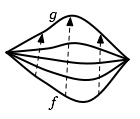
\includegraphics[scale = 0.5]{path_homotopy}\caption{A homotopy between $f$ and $g$.}\label{fig:homotopy}\end{marginfigure}

	For a subspace $A \subseteq X$, a relative homotopy is a homotopy with $H(a,t) = f(a) = g(a)$ for all $a \in A, t \in I$. 
	\end{Def}

\begin{Rem}
	Equivalently, we can specify a family of continuous maps $h_t \colon X \to Y$ such that $h_0 = f , h_1 = g$ and
\[
\begin{split}
H &\colon X \times I \to Y\\
 (x,t) &\mapsto h_t(x)
\end{split}
\]
is continuous. We will switch between the two equivalent definitions without comment, using whatever is more convenient. 
\end{Rem}
\begin{Prop}
For all spaces $X$ and $Y$, homotopy is an equivalence relation on the set of maps from $X$ to $Y$. Furthermore, if we are given $k \colon A \to X,\ell \colon Y \to B$ and homotopic maps $f \simeq g \colon X \to Y$, then $fk \simeq gk \colon A \to Y$ and $\ell f \simeq \ell g \colon X \to B$. 
\end{Prop}
\begin{proof}
Let $f,g \colon X \to Y$, then
\begin{enumerate}
	\item $f \simeq_F f$ via $F(x,t) = f(x)$ for all $x \in X,t \in I$. 
	\item If $f \simeq_F g$, then $g \simeq_G f$ where $G(x,t) = F(x,1-t)$. 
	\item If $f \simeq_F g$ and $g \simeq_G h$, then $f \simeq_H h$ via
	\[
H(x,t) = \begin{cases}
F(x,2t) & \text{ if } 0 \le t \le 1/2 \\
G(x,2t-1) & \text{ if } 1/2 \le t \le 1. 
\end{cases}
	\]
\end{enumerate}
For the last part of the proposition let $f_t$ be a homotopy between $f$ and $g$, then $f_tk$ and $\ell f_t$ give the required homotopy. 
\end{proof}
\begin{Def}
For a map $f \colon X \to Y$, we let $[f]$ denote the equivalence class containing $f$. The collection of all homotopy classes of maps from $X$ to $Y$ is denoted $[X,Y]$.\sidenote{If our spaces are based, then these should be homotopy classes of \emph{based} maps.} 
\end{Def}
\begin{Rem}
Note that if $\alpha = [f] \in [Y,Z]$ and $\beta = [g] \in [X,Y]$, then $\alpha\beta = [f \circ g] \in [X,Z]$, i.e., we can form the category $hTop_*$ whose objects are topological spaces, and whose morphisms are homotopy classes of maps. 
\end{Rem}
\begin{Rem}
We now very quickly review a number of standard topological constructions. 
\begin{itemize}
	\item Let $X$ be a space and $A \subseteq X$. A map $r \colon X \to A$ such that $ri(a) = a$ for all $a \in A$ is called a retraction of $X$ onto $A$, and $A$ is called a retract of $X$. 
	\item Let $i \colon A \hookrightarrow X$ be the inclusion, so that $ri = \text{id}_A$. If $ir \simeq \text{id}_X$, we call this a deformation retraction, and say that $A$ is a deformation retract of $X$. 
	\item If $f \colon X \to Y$, then a section of $f$ is a map $s \colon Y \to X$ such that $f \circ s = \text{id}_Y$. We can also ask for a \emph{homotopy} section by requiring only that $f \circ s \simeq \text{id}_Y$. 
\end{itemize}
\end{Rem}
\begin{Def}
A map $f \colon X \to Y$ is called null-homotopic if $f \colon c_y \colon X \to Y$ where $c_y X \to Y$ is the constant map sending all of $X$ to the point $y \in Y$. A homotopy between $f$ and $c_y$ is called a null-homotopy. A space $X$ is contractible if $\text{id}_X$ is null-homotopic. 
\end{Def}
\begin{Def}
Let $(X,x_0)$ be a based topological space and $X \times I$ the cylinder on $X$. The quotient
\[
CX = (X \times I)/(X \times \{ 1 \} \cup \{ x_0 \} \times I)
\]
with the base-point the equivalence class of $(x_0,1)$ is called the (reduced) cone on $X$. Note that we have a natural inclusion $X \to CX$ of based maps given by $x \mapsto [x,0]$. 
\end{Def}
\begin{Lem}\label{lem:cone_is_contractible}
The cone $CX$ is contractible. 
\end{Lem}
\begin{proof}
Define $F \colon CX \times I \to CX$ by
\[
F([x,t],s) = [x,s+(1-s)t]. 
\]
Note then that we have
\[
F([x,t],0) = [x,t] \quad \text{ and } \quad F([x,t],1) = [x,1]. \qedhere
\]

\end{proof}
\begin{Lem}\label{lem:extend_over_cone}
The following are equivalent:
\begin{enumerate}[label=(\roman*)]
	\item $f \colon X \to Y$ is null-homotopic. 
	\item $f$ can be extended to $CX$:
	% https://q.uiver.app/?q=WzAsMyxbMCwwLCJYIl0sWzEsMCwiWSJdLFswLDEsIkNYIl0sWzAsMSwiZiJdLFswLDIsImkiLDIseyJzdHlsZSI6eyJ0YWlsIjp7Im5hbWUiOiJob29rIiwic2lkZSI6InRvcCJ9fX1dLFsyLDEsIlxcZXhpc3RzIFxcdGlsZGUgZiIsMix7InN0eWxlIjp7ImJvZHkiOnsibmFtZSI6ImRhc2hlZCJ9fX1dXQ==
\[\begin{tikzcd}
	X & Y \\
	CX
	\arrow["f", from=1-1, to=1-2]
	\arrow["i"', hook, from=1-1, to=2-1]
	\arrow["{\exists \tilde f}"', dashed, from=2-1, to=1-2]
\end{tikzcd}\]
\end{enumerate}
\end{Lem}
\begin{proof}
$(i) \implies (ii): $ Suppose $f$ is null-homotopic, so $f \simeq_F \ast$. Then $F(X\times \{ 1 \} \cup \{ \ast \} \times I) = \ast$, so by the universal property of the quotient, we can find $\tilde F \colon CX \to Y$ such that $\tilde f \circ i = f$. 

$(ii) \implies (i): $ Suppose $\tilde f \circ i = f$, then because $CX$ is contractible (\Cref{lem:cone_is_contractible}), we have $f = \tilde f \circ \text{id}_{CX} \circ i \simeq \tilde f \circ (\ast_{CX}) \circ i \simeq \ast$, so that $f$ is null-homotopic. 
\end{proof}
\begin{Def}
A map $f \colon X \to Y$ is a homotopy equivalence if there exists $g \colon Y \to X$ such that $fg \simeq \text{id}_Y$ and $gf \simeq \text{id}_X$. We write $X \simeq Y$. 
\end{Def}
\begin{Exa}
\begin{enumerate}[label=(\roman*)]
	\item $X$ is contractible if and only if $X \simeq \ast$. 
	\item If $i \colon A \hookrightarrow X$, and $r \colon X \to A$ is a deformation retract, then $i$ and $r$ are homotopy equivalences, and $A \simeq X$. 
\end{enumerate}
\end{Exa}
\section{Higher homotopy groups}

\begin{Not} We will let $I_n = I^{\times n}, \partial I^n$ be the boundary of $I^n$, and write $[-,-]$ for homotopy classes of maps (if our spaces are based, these fix the base point).
\end{Not}
\begin{Def}
	For each $n \ge 0$ and $X$ a topological space with $x_0 \in X$, we define
	\[
\pi_n(X, x_0) = [(I^n, \partial I^n), (X, x_0)].
\]
\end{Def}
\begin{Rem}
	\begin{enumerate}[(i)]
		\item When $n = 0$, we have $I^0 = \text{pt}$ and $\partial I^0 = \emptyset$, therefore $\pi_0(X)$ is the set of path components of $X$.
		\item When $n = 1$, this is a group, but need not be abelian (for example, consider the wedge of two circles).
		\item Note that $I^n / \partial I^n \simeq S^n$ and $\partial I^n / \partial I^n \simeq s_0$. By the universal property of the quotient map, we see that 
		\[
		\pi_n(X, x_0) \cong [(S_n, s_0), (X, x_0)].
\]
	\end{enumerate}
\end{Rem}
\begin{Def}
	A maps of pairs $(X,A) \to (Y,B)$ is a map $f \colon X \to Y$ with $f(A) \subseteq B$, i.e., the diagram:
% https://q.uiver.app/?q=WzAsNCxbMCwwLCJBIl0sWzEsMCwiQiJdLFswLDEsIlgiXSxbMSwxLCJZIl0sWzAsMV0sWzIsMywiZiIsMl0sWzAsMiwiIiwxLHsic3R5bGUiOnsidGFpbCI6eyJuYW1lIjoiaG9vayIsInNpZGUiOiJib3R0b20ifX19XSxbMSwzLCIiLDEseyJzdHlsZSI6eyJ0YWlsIjp7Im5hbWUiOiJob29rIiwic2lkZSI6ImJvdHRvbSJ9fX1dXQ==
\[\begin{tikzcd}
	A & B \\
	X & Y
	\arrow[from=1-1, to=1-2]
	\arrow["f"', from=2-1, to=2-2]
	\arrow[hook', from=1-1, to=2-1]
	\arrow[hook', from=1-2, to=2-2]
\end{tikzcd}\]
	commutes. 
\end{Def}
\begin{Prop}
	If $n \ge 1$, then $\pi_n(X,x_0)$ is a group with respect to the operation
	\[
(f+g)(t_1,\ldots,t_n) = \begin{cases}
	f(2t_1,t_2,\ldots,t_n) & 0 \le t_1 \le 1/2 \\
	g(2t_1-1,t_2,\ldots,t_n) & 1/2 \le t_1 \le 1. 
\end{cases}
	\]
\end{Prop}
\begin{proof}
	The identity is given by the constant map taking all of $I^n$ to $x_0$ and the inverse of $f$ is given by 
	\[
-f(t_1,\ldots,t_n) = f(1-t_1,t_2,\ldots,t_n). \qedhere
	\]
\end{proof}
\begin{Rem}
	Call the group operation $+_1$. Note that we can also define an operation $+_i$ for $1 \le i \le n$ by the same formula on the $i$-th coordinate. 
\end{Rem}
\begin{Thm}
	All of these operations agree, and for $n \ge 2$, these give $\pi_n(X,x_0)$ the structure of an abelian group. 
\end{Thm}
This is a consequence of the following exercise, known as the Eckmann--Hilton lemma. 
\begin{exercise}{Eckmann--Hilton lemma}{}
	Let $M$ be a set and let $\ast,\bullet$ be two binary operations on $M$, $\ast,\bullet \colon M \times M \to M$, both with unit elements. Suppose that 
	\[
(a \ast b) \bullet (c \ast d) = (a \bullet c) \ast (b \bullet d)
	\]
	for all $a,b,c,d \in M$. Show that the units agree, these two operations agree, and that the multiplication is commutative and associative. 
\end{exercise}
\begin{Rem}
	Let use show that 
	\[
(f+_1 g) +_2 (h+_1 i) \simeq (f+_2 h) +_1 (g+_2 i). 
	\]
	Indeed, both of these are the following map
	\[
(t_1,t_2,\ldots,) \mapsto \begin{cases}
	f(2t_1,2t_2,\ldots,) &[1/2,0] \times [1/2,0]\\
	g(2t_1-2,2t_2,\ldots,) & [1/2,1] \times [0,1/2]\\
h(2t_1,2t_2-2,\ldots) & [0,1/2] \times [1/2,1]\\
i(2t_1-1,2t_2-2,\ldots) & [1/2,1] \times [1/2,1].
\end{cases}
	\]
\end{Rem}
\begin{Rem}
	Another approach is given by the following visualization: 
\begin{figure}[h!] \centering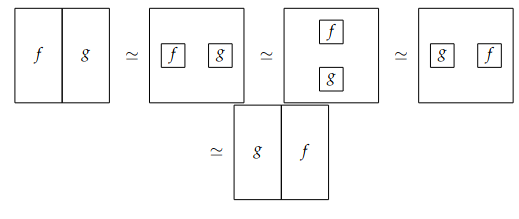
\includegraphics[scale = 0.5]{abelian.png}\caption{$f + g \simeq g +f $.}\label{fig:abelian}\end{figure}
	That is, so long as $n \ge 2$, we can shrink the domain of $f$ and $g$ to smaller cubes (mapping the remaining region to the base point), slide $f$ and $g$ past each other, and then increase the domains back again. 
\end{Rem}
\begin{exercise}{}{}
	Let $G$ be a topological group with identity element $e$, then $\pi_1(G,e)$ is abelian. \\
	\textbf{Hint: } Use Eckmann--Hilton, or note the following: A topological group is a group object in the category of topological spaces. What is a group object in the category of groups? 
\end{exercise}
\begin{Prop}
	If $n \ge 1$ and $X$ is path connected, then there is an isomorphism $\beta_{\gamma} : \pi_n(X, x_0) \xrightarrow{\simeq} \pi_n(X, x_0)$ given by $\beta_{\gamma}([ f ]) = [\gamma \circ f ]$ where $\gamma$ is a path in $X$ from $x_1$ to $x_0$ and $\gamma \circ f$ is constructed by first shrinking the domain of $f$ to a smaller cube inside of $I^n$, and then inserting the path $\gamma$ radially from $x_1$ to $x_0$ on the boundaries of these cubes.
	\begin{figure}[h] \centering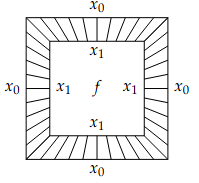
\includegraphics[scale = 0.5]{path.png}\caption{$\beta_{\gamma}$.}\label{fig:path}\end{figure}
\end{Prop}
\begin{proof}
	Observe the following:
	\begin{enumerate}
		\item $\gamma \circ (f + g) \simeq \gamma \circ f + \gamma \circ g$, i.e., $\beta_{\gamma}$ is a group homomorphism.
		\item $(\gamma \circ \eta) \circ f \simeq \gamma \circ (\eta \circ f)$, for $\eta$ a path from $x_0$ to $x_1$. 
		\item $c_{x_0} \circ f \simeq f$, where $c_{x_0}$ denotes the constant path based at $x_0$. 
		\item $\beta_{\gamma}$ is well-defined with respect to homotopies of $f$ or $\gamma$. 
	\end{enumerate}

	The only point that is perhaps not clear is (i). For this, we deform $f$ and $g$ to be constant on the right and left halves of $I^n$, respectively, producing maps we call $f+0$ and $0 + g$. We then excise a wider symmetric middle slab of $\gamma(f+0)$  and $\gamma(0+g)$ until it becomes $\gamma(f+g)$:
\begin{figure}[h] \centering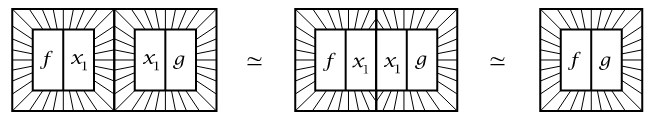
\includegraphics[scale = 0.5]{path_invariance.png}\end{figure}
\end{proof}
\begin{Rem}
	Therefore if $X$ is path-connected, different choices of base point $x_0$ yield isomorphic groups $\pi_n(X,x_0)$, which may then simply be written as $\pi_n(X)$. 
\end{Rem}
\begin{Lem}
	If $\{ X_{\alpha} \}$ is a collection of path-connected spaces, then $\pi_n(\prod_{\alpha} X_{\alpha}) \cong \prod_{\alpha} \pi_n(X_{\alpha})$. 
\end{Lem}
\begin{proof}
	Note that $\Hom(Y,\prod_{\alpha} X_{\alpha}) \simeq \prod_{\alpha} \Hom(Y,X_{\alpha})$. In particular, a map $S^n \to \Hom(Y,\prod_{\alpha}X_{\alpha})$ is determined by a collection of maps $S^n \to X_{\alpha}$. Likewise, a homotopy $S^n \times I \to \prod_{\alpha} X_{\alpha}$ is determined by a colletion of homotopies $S^n \times I \to X_{\alpha}$. This implies the result. 
\end{proof}
\begin{Prop}
	Homotopy groups are functorial: given a map $\phi \colon X \to Y$ we get group homomorphisms $\phi_{\ast} \colon \pi_n(X,x_0) \to \pi_n(X,\phi(x_0))$ given by $[f] \mapsto [\phi \circ f]$ for all $n \ge 1$. 
\end{Prop}
\begin{proof}
We have the following:
	\begin{enumerate}
	\item $\phi_*$ is well-defined: if $f \simeq g$ via $\psi_t$, then $\phi \circ \psi_t$ defines a homotopy between $\phi \circ f$ and $\phi \circ g$. 
	\item This is a group homomorphism: $\phi \circ (f+g) \simeq \phi \circ g + \phi \circ g$ by the definition of the addition operation. Therefore. 
	\[
\phi_*[f+g] = \phi_*[f] + \phi_*[g]. 
	\]
\end{enumerate}
\end{proof}
\begin{exercise}{}{}
	If $\phi \colon X \to Y$ is homotopy equivalence (not necessarily base-point preserving), then $\pi_* \colon \pi_n(X,x_0) \to \pi_n(Y,\phi(y_0))$ is an isomorphism.  
\end{exercise}
\begin{Rem}
	We recall the following lifting property: Suppose $p \colon (\tilde X,\tilde x_0) \to (X,x_0)$ is a covering, and there is a map $f \colon (Y,y_0) \to (X,x_0)$ with $Y$ path-connected and locally path-connected. Then a lift $\tilde f$ exists if and only if $f_*\pi_1(Y,y_0) \subseteq p_*\pi_1(\tilde X,\tilde x_0)$. 
	% https://q.uiver.app/?q=WzAsMyxbMCwxLCIoWSxZXzApIl0sWzEsMSwiKFgseF8wKSJdLFsxLDAsIihcXHRpbGRlIFgseF8wKSJdLFswLDEsImYiXSxbMiwxXSxbMCwyLCJcXHRpbGRlIGYiLDAseyJzdHlsZSI6eyJib2R5Ijp7Im5hbWUiOiJkYXNoZWQifX19XV0=
\[\begin{tikzcd}
	& {(\tilde X,\tilde x_0)} \\
	{(Y,y_0)} & {(X,x_0)}
	\arrow["f", from=2-1, to=2-2]
	\arrow["p",from=1-2, to=2-2]
	\arrow["{\tilde f}", dashed, from=2-1, to=1-2]
\end{tikzcd}\]

\end{Rem}
\begin{Prop}
	If $p$ is a covering, then $p_* \colon \pi_n(\tilde X,\tilde x_0) \to \pi_n(X,x_0)$ is an isomorphism for all $ n \ge 2$. 
\end{Prop}
\begin{proof}
Let us first show surjectivity. To that end, suppose we have a map $f \colon (S^n,s_0) \to (X,x_0)$ where $n \ge 2$. The assumption on  $n$ gives $\pi_1(S^n) = 0$, so $f_*\pi_1(S^n,s_0) \subseteq p_*\pi_1(\tilde X,\tilde x_0)$ holds. We therefore find a lift in the following:
\[\begin{tikzcd}
	& {(\tilde X,\tilde x_0)} \\
	{(S^n,s_0)} & {(X,x_0)}
	\arrow["f", from=2-1, to=2-2]
	\arrow["p", from=1-2, to=2-2]
	\arrow["{\tilde f}", dashed, from=2-1, to=1-2]
\end{tikzcd}\]
Then $p_*[\tilde f] = [f]$, and $p_*$ is surjective. 

To see that $p_*$ is injective, let $[\tilde f] \in \ker(p_*)$, i.e., $p_*[\tilde f] = [p \circ \tilde f] = 0$. Let $f = p \circ \tilde f$, then this is homotopic to the constant map $f \simeq c_{x_0}$ via a homotopy $\phi_t \colon (S^n,s_0) \to (X,x_0)$ with $\phi_1 =f $ and $\phi_0 = c_{x_0}$. By the same argument as above, the homotopy $\phi_t$ can be lifted to $\tilde \phi_t$. This satisfies $p \circ \tilde \phi_1 \simeq \phi_1 $ and $p \circ \tilde \phi_0 \simeq \phi_0$. By the uniqueness of lifts, we must have $\tilde \phi_1 \simeq \tilde f$ and $\tilde \phi_0 \simeq c_{x_0}$. In other words, $\tilde \phi_t$ gives a homotopy between $\tilde f$ and $c_{x_0}$, so that $[\tilde f]  = 0$, and $p_*$ is injective. 
\end{proof}
\begin{Exa}\label{ex:s1}
	$S^1$ has universal cover $p \colon \mathbb{R} \to S^1$, $p(t) = e^{2\pi i t}$. Then $\pi_n(S^1) \cong \pi_n(\mathbb{R}) \cong 0$ for $n \ge 2$. 
\end{Exa}
\begin{exercise}{}{}
	Find two spaces $X,Y$ with $\pi_nX \cong \pi_nY$ but $X \not \simeq Y$. 

	\textbf{Hint: } What is the universal cover of $\mathbb{R}P^n$?
\end{exercise}
\begin{Rem}[Relative homotopy groups]
	Suppose we have $(X,x_0)$ and a subspace $A$ containing $x_0$. We note that $i_* \colon \pi_n(A,x_0) \to \pi_n(X,x_0)$ is not injective in general (example, take $S^1$ into $\mathbb{R}^2$). An element in the kernel of $i_*$ is a map $f \colon (I^n,\partial I^n) \to (A,x_0)$ such that 
	\[
(I^n,\partial I^n) \xrightarrow{f} (A,x_0) \xrightarrow{i} (X,x_0)
	\] 
	is homotopic to $c_{x_0}$. This means there exists a homotopy
	\[
H \colon I^n \times I \to X
	\]
	such that $H(-,1) = f, H(-,0) = c_{x_0}$ and $H \mid_{\partial I^n \times I} = c_{x_0}$. 

	If we define $J^n = I^n \times \{ 0 \} \cup \partial I^n \times I \subseteq I^n \times I$, then this is a map of triples
	\[
H \colon (I^{n+1},\partial I^{n+1},J^n) \to (X,A,x_0). 
	\] 
\end{Rem}
\begin{Def}
	\[
\pi_n(X,A,x_0) = [(I^n,\partial I^n,J^{n-1}),(X,A,x_0)]
	\]
\end{Def}
\begin{Rem}
	Equivalently, 
	\[
\pi_n(X,A,x_0) = [(D^n,S^{n-1},s_0),(X,A,x_0)]
	\]
\end{Rem}
\begin{Prop}
	If $n \ge 2$, then $\pi_n(X,A,x_0)$ is a group, and if $n \ge 3$, then it is abelian. 

	For all $n \ge 2$, a map of pairs $\phi \colon (X,A,x_0) \to (Y,B,y_0)$ induces homomorphisms $\phi_* \colon \pi_n(X,A,x_0) \to \pi_n(Y,B,y_0)$ for all $n \ge 2$. 
\end{Prop}
\begin{proof}
This is similar to the case of $\pi_n(X)$ itself, and the details are left to the reader. 
\end{proof}
\begin{Thm}\label{thm:les_rel}
	The relative homotopy groups $(X,A,x_0)$ fit into a long exact sequence 
	\[
\cdots \to \pi_n(A,x_0) \xr{i_*} \pi_n(X,x_0) \xr{j_*} \pi_n(X,A,x_0) \xr{\partial_n} \pi_{n-1}(A,x_0) \to \cdots
	\]
	where the map $\partial_n$ is defined by $\partial_n([f]) = [f\mid_{I^{n-1}}]$. 
\end{Thm}
The proof relies on the following.
\begin{Lem}[Compression criterion]\label{lem:compression}
	A map $f \colon (D^n,S^{n-1},x_0) \to (X,A,x_0)$ represents 0 in $\pi_n(X,A,x_0)$ if and only if $f \sim g \text{ rel } S^{n-1}$, where $g$ is a map whose image is contained entirely in $A$. 
\end{Lem}
\begin{proof}
	Suppose $[f] = [g]$ with $g$ as in the statement of the lemma. Note that there is a deformation of $D^n$ onto $x_0$, and so $[f] = [g] = 0$ in $\pi_n(X,A,x_0)$. 

	Conversely, suppose that $[f]$ represents 0 in $\pi_n(X,A,x_0)$. This means there exists a homotopy, relative to $S^{n-1}$, $F \colon D^n \times I \to X$ with $F \mid_{D^n \times \{0 \}} = f$, $F \mid_{D^n \times 1} = c_{x_0}$ and $F \mid_{S^{n-1} \times I} \subseteq A$. We can restrict $F$ to a family of $n$-disks in $D^n \times I$ starting with $D^n \times \{ 0 \}$ and ending with the disk $D^n \times \{1 \} \cup S^{n-1} \times \{ 1\}$, all the disks in the family having the same boundary, then we get a homotopy from $f$ to a map in $A$, stationary on $S^{n-1}$ (said in other words, we can deformation retract $D^n \times [0,1]$ onto $D^n \times \{1 \} \cup S^{n-1} \times I$). 
\end{proof}
We now prove the existence of the long exact sequence.\sidenote{This is the type of proof that is best done by the reader themselves.}
\begin{proof}[Proof of \Cref{thm:les_rel}]
	\textbf{Step 1. }Let us first show exactness at $\pi_n(X,x_0)$. \\

	We first show $\im(i_*) \subseteq \ker(j_*)$. Note that $j_*i_*$ is induced by the composition $j \circ i$ and that these are both inclusion maps. Therefore, for $[f] \in \pi_n(A,x_0)$ we have $j_*i_*[f] = [j \circ i \circ f]$, but this has image contained in $A$, and so $j_*i_*[f] = 0$. This shows $\im(i_*) \subseteq \ker(j_*)$. 

	To see the converse (namely, $\ker(j_*) \subseteq \im(i_*)$) let $[f] \in \ker(j_*)$, i.e. $[j \circ f] = 0$. Note that again $j$ is an inclusion map, and by the compression criteria $f \simeq g'$ relative to $S^{n-1}$, where $g'$ has image contained in $A$. Since $x_0 \in S^{n-1}$, the homotopy fixes the basepoint, i.e, $[f] = [g'] \in \pi_n(X,x_0)$. But because $g'$ has image in $A$, $[g'] \in \pi_n(A,x_0)$ and $i_*[g'] = [i \circ g'] = [f]$, so $[f] \in \im(i_*)$. 

	\textbf{Step 2. } Let us now show exactness at $\pi_n(X,A,x_0)$. \\

	Note that the composite $\partial \circ j_* = 0$ since the restriction of a map $(I^n,\partial I^n,J^{n-1}) \to (X,x_0,x_0)$ to $I^{n-1}$ has image $x_0$ and so represents $0$ in $\pi_{n-1}(A,x_0)$. Therefore, $\im(j_*) \subseteq \ker(\partial)$. For the converse, suppose $[f] \in \ker(\partial)$. This means there exists a basepoint preserving homotopy $H \colon I^{n-1} \times I \to A$ (relative to $\partial I^{n-1}$) from $f \mid_{I^{n-1} \times \{ 0 \}}$ to the constant map where the image of $H$ is contained entirely in $A$. We can then define another homotopy $H$, such that $G_0 = f$, $G_t \mid_{I^{n-1}} = H_t$ and the rest of the image of $G_t$ is $f[I^n]$ union with the image of $H_s$ for $0 \le s \le t$. This homotopy maps $S^{n-1}$ into $A$ at all times, so $[f] = [G_1]$. Moreover, $G_1$ maps the boundary of $I^n$ to $x_0$, so $[G_1] \in \pi_n(X,x_0)$. Altogether, 
	\[
j_*[G_1] = [j \circ G_1] = [G_1] = [f]
	\]
	so $\ker(\partial) \subseteq \im(j_*)$. 


\textbf{Step 3:} Exactness at $\pi_n(A,x_0)$.
	
	Let $[f] \in \pi_n(X,A,x_0)$ then $i_*\partial \in \pi_{n-1}(X,x_0)$ is the class represented by $f \mid_{I^{n-1}}$ and this is homotopic relative $J^{n-2}$ to the constant map to $x_0$, via $f$ viewed as a homotopy. So this implies $\im(\partial_*) \subseteq \ker(i_*)$. Conversely, let $[f] \in \ker(i_*)$ i.e., $i_*[f]= [i \circ f]= 0$. Therefore, there exists a homotopy $H$ between $f$ and a constant map through a homotopy that has image in $X$ and preserves $x_0$. Since $H_0 = f$ has image in $A$ and $H_1$ has image $\{x_0\}$, and $H_0$ takes the boundary to $\{ x_0 \}$, we see that $[H] \in \pi_n(X,A,x_0)$, and moreover $\partial([H]) \simeq f$. Therefore, $[f] \in \im(\partial)$, and $\im(\partial) = \ker(i_*)$. 
\end{proof}
\begin{Def}
	A pair $(X,A)$ with basepoint $x_0$ is said to be $n$-connected if $\pi_i(X,A) = 0$ for all $i \le n$.\footnote{A 0-connected space is exactly a path-connected space.}
\end{Def}
\begin{Lem}
	A pair $(X,A)$ is $n$-connected if and only if $\pi_i(A) \xr{i_*} \pi_i(X)$ is an isomorphism for $i < n$ and a surjection for $i = n$. 
\end{Lem}
\begin{proof}
	Use the long exact sequence in homotopy. 
\end{proof}
\begin{exercise}{}{}
Let $X$ be a path-connected space, and $CX$ the cone on $X$. Show that 
	\[
\pi_n(CX,X,X_0) \cong \pi_{n-1}(X,x_0)
	\]
	for $n \ge 1$. 
\end{exercise}
\section{Cofibrations and the homotopy extension property}
\begin{Def}
Let $\cat C$ be a class of topological spaces. A map $i \colon A \to X$ has the homotopy extension property (HEP) if, for every $Y \in \cat C$, the following extension property has a solution\sidenote{Here $i_0(x) = (x,0)$.}
% https://q.uiver.app/?q=WzAsNSxbMCwwLCJBIl0sWzAsMSwiWCJdLFsxLDAsIkEgXFx0aW1lcyBJIl0sWzEsMSwiWCBcXHRpbWVzIEkiXSxbMiwyLCJYIl0sWzAsMSwiaSIsMl0sWzAsMiwiIiwwLHsic3R5bGUiOnsidGFpbCI6eyJuYW1lIjoiaG9vayIsInNpZGUiOiJ0b3AifX19XSxbMSwzLCJpXzAiLDIseyJzdHlsZSI6eyJ0YWlsIjp7Im5hbWUiOiJob29rIiwic2lkZSI6InRvcCJ9fX1dLFsyLDMsImYgXFx0aW1lcyBcXHRleHR7aWR9Il0sWzIsNCwiSCIsMCx7ImN1cnZlIjotM31dLFsxLDQsImYiLDIseyJjdXJ2ZSI6M31dLFszLDQsIlxcZXhpc3RzIFxcdGlsZGUgSCIsMCx7InN0eWxlIjp7ImJvZHkiOnsibmFtZSI6ImRhc2hlZCJ9fX1dXQ==
\[\begin{tikzcd}
	A & {A \times I} \\
	X & {X \times I} \\
	&& Y
	\arrow["i"', from=1-1, to=2-1]
	\arrow["i_0", hook, from=1-1, to=1-2]
	\arrow["{i_0}"', hook, from=2-1, to=2-2]
	\arrow["{i \times \text{id}}", from=1-2, to=2-2]
	\arrow["H", curve={height=-18pt}, from=1-2, to=3-3]
	\arrow["f"', curve={height=18pt}, from=2-1, to=3-3]
	\arrow["{\exists \tilde H}", dashed, from=2-2, to=3-3]
\end{tikzcd}\]
A map $f \colon A \to X$ is a cofibration if it has the HEP with respect to all spaces $Y$.\sidenote{We will see later that cofibrations are always inclusions, and, if $X$ is Hausdorff, are always closed maps.}
\end{Def}
\begin{Rem}
Note that we do not ask that $\tilde H$ is unique. 
\end{Rem}
\begin{Rem}\label{Rem:hep_adjoint}
If we are in a 'nice' category of topological spaces (see CREF), which we always assume, then we have an adjunction
\[
\Hom(X,\Hom(Y,Z)) \cong \Hom(X \otimes Y,Z)
\]
of topological spaces, where $\Hom(Y,Z)$ is given the compact open topology. Writing, $Z^Y \coloneqq \Hom(Y,Z)$, the homotopy extension property admits a reformulation in the following diagram
% https://q.uiver.app/?q=WzAsNCxbMCwwLCJBIl0sWzEsMCwiWV5JIl0sWzAsMSwiWCJdLFsxLDEsIlkiXSxbMCwxLCJoIl0sWzAsMiwiaSIsMl0sWzIsMywiZiIsMl0sWzEsMywicCJdLFsyLDEsIlxcdGlsZGUgaCIsMCx7InN0eWxlIjp7ImJvZHkiOnsibmFtZSI6ImRhc2hlZCJ9fX1dXQ==
\[\begin{tikzcd}
	A & {Y^I} \\
	X & Y
	\arrow["h", from=1-1, to=1-2]
	\arrow["i"', from=1-1, to=2-1]
	\arrow["f"', from=2-1, to=2-2]
	\arrow["p", from=1-2, to=2-2]
	\arrow["{\exists \tilde h}", dashed, from=2-1, to=1-2]
\end{tikzcd}\]
where $p \colon Y^I \to Y$ is the evaluation at 0 map. It is often easier to work with this equivalent diagram. 
\end{Rem}
\begin{exercise}{}{}
Let $(X,A)$ have the HEP, and assume moreover that $i \colon A \to X$ is a retract up to homotopy. Show that $A$ is a retract of $X$. 
\end{exercise}
\begin{Lem}
	Let $J = [0,1]$. 
	\begin{enumerate}[label=(\roman*)]
		\item The inclusion $i_0 \colon X \to X \times J$ has the homotopy extension property for all $Y$. 
		\item The inclusion $i_0 \colon X \to CX$ has the homotopy extension property for all $Y$.   
	\end{enumerate}
\end{Lem}
\begin{proof}
	The proof in both cases is very similar; we do the first case in some detail. We are claiming there exists a lift $\tilde H$ in the following diagram:
	\[\begin{tikzcd}
	X & {X \times I} \\
	X \times J & {X \times J \times I} \\
	&& Y
	\arrow["i"', from=1-1, to=2-1]
	\arrow["i_0", hook, from=1-1, to=1-2]
	\arrow["{i_0}"', hook, from=2-1, to=2-2]
	\arrow["{i \times \text{id}}", from=1-2, to=2-2]
	\arrow["H", curve={height=-18pt}, from=1-2, to=3-3]
	\arrow["f"', curve={height=18pt}, from=2-1, to=3-3]
	\arrow["{\exists \tilde H}", dashed, from=2-2, to=3-3]
\end{tikzcd}\]
Geometrically, we will do this in two parts: we will define a map that "stacks" the two intervals on top of each other, i.e., we construct a map $G \colon X \times J \times I \to X \times [0,2]$. We will then do $H$ on one part of the cylinder, and $f$ on the remaining part. 

For the first part, let $G \colon X \times J \times I \to X \times [0,2]$ be defined as\sidenote{To see what is going on it is worth testing some cases and drawing pictures. For example, when $t = 0$ we have $G(x,0,s) =  (x,0)$. When $t = 1$ we have $G(x,1,s) = (x,1+s)$. When $s = 0$ we have $G(x,t,0) = (x,t)$ and when $s = 1$ we have $G(x,t,1) = (x,2t)$.}
\[
G(x,t,s) = (x,t(1+s)). 
\]
We then define $F \colon X \times [0,2] \to Y$ by
\[
F(x,k) = \begin{cases}
	f(x,k) & 0 \le k \le 1 \\
	H(x,k/2) & 1 \le k \le 2. 
\end{cases}
\]
Putting these together and defining $\tilde H \coloneqq F \circ G$, we see that\sidenote{Again, it is worthwhile to consider some cases. For example, if $t = 0$, then $(1-t)(1+s) = (1+s) \ge 1$ for all $s$, so $\tilde H((x,0),s) = H(x,s)$. At the other extreme, if $t =1$, then $(1-t)(1+s) = 0 \le 1$ for all $s$, so $\tilde H((x,1),s) = f(x,1)$. }
\[
\tilde H((x,t),s) = \begin{cases}
f(x,1-(1-t)(1+s)), & (1-t)(1+s) \le 1 \\
H(x,(1-t)(1+s)-1), & (1-t)(1+s) \ge 1. 
\end{cases}
\]
One verifies directly that this gives the required extension. 
\end{proof}
\begin{Rem}
We recall that given a map $f \colon X \to Y$, the mapping cylinder (see \Cref{fig_mapping_cylinder}) is the pushout\begin{marginfigure}[5\baselineskip] \centering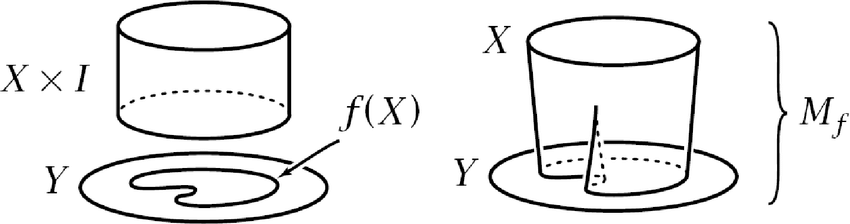
\includegraphics[scale = 0.2]{map_cylinder.png}\caption{The mapping cylinder.}\label{fig_mapping_cylinder}\end{marginfigure}
% https://q.uiver.app/?q=WzAsNCxbMCwwLCJYIl0sWzAsMSwiWSJdLFsxLDEsIk1fZiJdLFsxLDAsIlggXFx0aW1lcyBJIl0sWzAsMSwiZiIsMl0sWzEsMl0sWzAsMywiaV8xIl0sWzMsMl0sWzIsMCwiIiwxLHsic3R5bGUiOnsibmFtZSI6ImNvcm5lci1pbnZlcnNlIn19XV0=
\[\begin{tikzcd}
	X & {X \times I} \\
	Y & {M_f}
	\arrow["f"', from=1-1, to=2-1]
	\arrow[from=2-1, to=2-2]
	\arrow["{i_0}", from=1-1, to=1-2]
	\arrow[from=1-2, to=2-2]
	\arrow["\ulcorner"{anchor=center, pos=0.125, rotate=180}, draw=none, from=2-2, to=1-1]
\end{tikzcd}\]
In formulas, 
\[
M_f = ((X \times I) \coprod Y)/((0,x) \sim f(x), \hspace{1mm} \forall x \in X)
\]

Note that $M_f$ deformation retracts on $Y$ by sliding each point $(x,t) \in M_f$ to the end-point. Note that we have a natural map $j \colon X \to M_f$ sending $x$ to $(x,1)$.
\end{Rem}
\begin{Lem}
The map $j \colon X \to M_f$ has the HEP for all spaces $Y$.
\end{Lem}
\begin{proof}
The proof is similar to the previous lemma; one just has to modify the end point by defining
\[
\tilde H|_{Y \times I}(y,s) = f(y,0). 
\]
\end{proof}
\begin{Cor}\label{cor:spheres_are_cofibrations}
The inclusion $S^{n-1} \to D^n$ is a cofibration. 
\end{Cor}
\begin{proof}
	Simply note that $D^n \simeq CS^{n-1}$. 
\end{proof}
There is a universal test space for cofibrations. 
\begin{Prop}\label{prop:universal_cofibration}
	Let $i \colon A \to X$, and let $M_i$ be the mapping cylinder. Then $i \colon A \to X$ is a cofibration if and only if there exists a map $r \colon X \times I \to M_i$ making the diagram
% https://q.uiver.app/?q=WzAsNSxbMCwwLCJBIl0sWzAsMiwiWCJdLFsyLDIsIk1faSJdLFsyLDAsIkEgXFx0aW1lcyBJIl0sWzEsMSwiWCBcXHRpbWVzIEkiXSxbMCwxLCJpIiwyXSxbMSwyXSxbMCwzLCJpXzAiXSxbMywyXSxbMiwwLCIiLDEseyJzdHlsZSI6eyJuYW1lIjoiY29ybmVyLWludmVyc2UifX1dLFsxLDQsImlfMCIsMl0sWzMsNCwiaSBcXHRpbWVzIFxcdGV4dHtpZH0iLDJdLFs0LDIsIlxcZXhpc3RzIHIiLDAseyJzdHlsZSI6eyJib2R5Ijp7Im5hbWUiOiJkYXNoZWQifX19XV0=
\[\begin{tikzcd}
	A && {A \times I} \\
	& {X \times I} \\
	X && {M_i}
	\arrow["i"', from=1-1, to=3-1]
	\arrow[from=3-1, to=3-3]
	\arrow["{i_0}", from=1-1, to=1-3]
	\arrow[from=1-3, to=3-3]
	\arrow["\ulcorner"{anchor=center, pos=0.125, rotate=180}, draw=none, from=3-3, to=1-1]
	\arrow["{i_0}"', from=3-1, to=2-2]
	\arrow["{i \times \text{id}}"', from=1-3, to=2-2]
	\arrow["{\exists r}", dashed, from=2-2, to=3-3]
\end{tikzcd}\]
commute. 
\end{Prop}
\begin{proof}
If $i$ is a cofibration, then the map $r$ exists as a consequence of the HEP. 

For the other direction, if $r$ exists, then for any maps $f \colon X \to Y$ and $H \colon A \times I \to Y$ making the obvious diagram commute, the universal property of the pushout gives us a map $H' \colon M_i \to Y$. Then let $\tilde H = H' \circ r$, and we are done. 
\end{proof}
\begin{Cor}\label{cor:cofibration_retract}
If $A \subseteq X$, then $I \colon A \to X$ is a cofibration if and only if $X \times I$ is a retract of $M_i = X \times \{ 0 \} \cup A \times I$. 
\end{Cor}
\begin{Cor}
A cofibration $i \colon A \to X$ is an injection. If $X$ is Hausdorff, then $i(A)$ is closed in $X$. 
\end{Cor}
\begin{proof}
Let $J \colon A \times I \to M_i$ be the canonical map (arising from the definition of $M_i$ as a pushout). Then, $J(a,1) = r(i(a),1)$, and observe that $J\mid_{A \times \{ 1 \}}$ is the identity, as it is the top of the mapping cylinder. So, $i(a) \ne i(a')$ if $a \ne a'$, i.e., $i$ is injective. 

Because $i \colon A \to X$ is a cofibration, so is $i(A) \to X$. Hence $X \times I$ retracts onto $X \times \{ 0 \} \cup i(A) \times I$ (\Cref{cor:cofibration_retract}). For a Hausdorff space, the image of a retract is closed, and so $X \times \{ 0 \} \cup i(A) \times I$ is a closed subspace of $X \times I$. Intersecting with $X \times \{ 1 \}$, we see that $i(A) \times \{ 1 \}$ is closed in $X \times \{ 1 \}$, i.e, $i(A)$ is closed in $X$.  
\end{proof}
The following (rather pathological) example shows that $i$ is not always a closed map if $X$ is not Hausdorff. 
\begin{exercise}{}{}
Let $A = \{ a \}$ and $X = \{ a , b\}$ with the trivial topology. Show that the inclusion $A \to X$ is a cofibration whose image is not closed. 
\end{exercise}
\begin{Rem}
The next goal is to show that CW-complexes $(X,A)$ are always cofibrations. The key is the following exercise. 
\end{Rem}
\begin{exercise}{}{}
\begin{enumerate}[label=(\alph*)]
  	\item Suppose $\{ (X_i,A_i)\}$ are a collection of spaces satisfying the HEP, then so does $\{ (\coprod X_i, \coprod A_i) \}$.
  	\item Suppose $(X,A)$ satisfies the HEP, and $f \colon A \to B$ is a continuous map. Let $Y = X \cup_f B$ be the pushout, then $(Y,B)$ satisfies the HEP. 
  	\item Suppose $A = X_0 \subseteq X_1 \subseteq \cdots \subseteq X_n \subseteq X_{n+1} \subseteq \cdots$.

  	Let $X = \colim X_i$. If each $(X_i,X_{i-1})$ satisfies the HEP, then so does $(X,A)$. 
  \end{enumerate}  
\end{exercise}

\begin{Thm}
A relative $CW$-complex $(X,A)$ satisfies the HEP. 
\end{Thm}
\begin{proof}
Using \Cref{cor:spheres_are_cofibrations} and the previous exercise we see that $(S^{n-1},D^n)$ satisfies the HEP $\implies (\coprod S^{n-1},\coprod D^n)$ satisfies the HEP. Inductively, $(X_{n-1},A)$ satisfies the HEP and by the exercise $(X,A)$ satisfies the HEP. 
\end{proof}
\begin{Rem}
One can also prove this directly by constructing a deformation retract $r \colon X \times I \to X \times \{ 0 \} \cup A \times I$. 
\end{Rem}
\begin{Rem}
One can consider the following question: Suppose that $A \subset X$ with $A$ contractible, then is $X \simeq X/A$? Surprisingly, this is not true in general. Indeed, let $A = S^1 \setminus \{ (1,0) \}$ and consider $A \to S^1$. Then $S^1/A \cong T$, the $T = \{ a ,b \}$ the two point space with open sets $\emptyset, \{ a \}, \{ a, b\}$ (this is the Sierpi\'nski space). One can check that this space is contractible.\sidenote{See \url{https://math.stackexchange.com/a/264789/64273}.} The exact condition we need is that $A \to X$ is a cofibration. 
\end{Rem}
\begin{Def}
A contracting homotopy is a map $H \colon X \times I \to X$ such that $H(x,0) = \text{id}_X$ and $H(x,1) = c_{x_0}$, the constant map at $x_0$. 
\end{Def}
\begin{Prop}\label{prop:quotient_contractible}
Suppose $A \subseteq X$ and $x_0 \in A$. Suppose there exists a map $H \colon X \times I \to X$ such that $H \mid_{X \times \{ 0 \}} = \text{id}_X$ and $H \mid_{A \times I}$ has image in $A$ and is a contacting homotopy for $A$. Then $q \colon X \to X/A$ is a homotopy equivalence. 
\end{Prop}
\begin{proof}
We need to find $p \colon X/A \to X$ such that $q \circ p \simeq \text{id}_{X/A}$ and $p \circ q \simeq \text{id}_X$. The quotient map has a set-theoretic section given by 
\[
s(\overline x) = \begin{cases}
	x & x \not\in A\\
	x_0 & x \in A
\end{cases}
\]
Define $p \colon X/A \to X$ by the following diagram
% https://q.uiver.app/?q=WzAsNCxbMCwwLCJYIl0sWzEsMCwiWC9BIl0sWzIsMCwiWCJdLFsyLDEsIlgiXSxbMCwxLCJxIl0sWzEsMiwicyJdLFsyLDMsIkggXFxtaWRfe1ggXFx0aW1lcyBcXHsgMSBcXH19Il0sWzEsMywicCIsMl1d
\[\begin{tikzcd}
	X & {X/A} & X \\
	&& X
	\arrow["q", from=1-1, to=1-2]
	\arrow["s", from=1-2, to=1-3]
	\arrow["{H \mid_{X \times \{ 1 \}}}", from=1-3, to=2-3]
	\arrow["p"', from=1-2, to=2-3]
\end{tikzcd}\]
Assume for a moment that $p$ is continuous. Then $p \circ q = H\mid_{X \times \{ 1 \}}$, and so $H$ gives a homotopy between $\text{id}_X$ and $p \circ q = H \mid_{X \times \{ 1 \}}$. Likewise, if we define $G$ by 
% https://q.uiver.app/?q=WzAsNCxbMCwwLCJYL0EgXFx0aW1lcyBJIl0sWzEsMCwiWCBcXHRpbWVzIEkiXSxbMiwwLCJYIl0sWzIsMSwiWC9BIl0sWzAsMSwicyBcXHRpbWVzIFxcdGV4dHtpZH0iXSxbMSwyLCJIIl0sWzIsMywicSJdLFswLDMsIkciLDJdXQ==
\[\begin{tikzcd}
	{X/A \times I} & {X \times I} & X \\
	&& {X/A}
	\arrow["{s \times \text{id}}", from=1-1, to=1-2]
	\arrow["H", from=1-2, to=1-3]
	\arrow["q", from=1-3, to=2-3]
	\arrow["G"', from=1-1, to=2-3]
\end{tikzcd}\]
and assume that $G$ is continuous, then 
\[
G(\overline x,1) = q \circ (H\mid_{X \times \{ 1 \}} \circ s) = q \circ p,
\]
so that $G$ is a homotopy between $\text{id}_{X/A}$ and $q \circ p$. To see that $p$ is continuous, let $U \subset X$ be open, then 
\[
q^{-1}p^{-1}(U) = (p \circ q)^{-1}(U) = (H \mid_{X \times \{ 1\}})^{-1}(U)
\]
is open in $X$ by the continuity of $H \mid_{X \times \{ 1\}}$, hence $p^{-1}(U)$ is open in $X/A$ by the definition of the quotient topology, and so $p$ is continuous. We leave the proof of continuity of $G$ to the reader. 
\end{proof}
\begin{Thm}\label{thm:quotient_cofibration}
Let $A \subseteq X$ be a subspace with $A$ contractible. Suppose that the inclusion $i \colon A \to X$ is a cofibration, then $X \to X/A$ is a homotopy equivalence. 
\end{Thm}
\begin{proof}
	Let $h \colon A \to I \to A$ be a contracting homotopy. Let $H \colon A \times I \to X$ be the composition of $h$ with the inclusion map of $A$ into $X$, i.e., the following diagram commutes:
	\[\begin{tikzcd}
	A & {A \times I} \\
	X & {X \times I} \\
	&& X
	\arrow["i"', from=1-1, to=2-1]
	\arrow["i_0", hook, from=1-1, to=1-2]
	\arrow["{i_0}"', hook, from=2-1, to=2-2]
	\arrow["{i \times \text{id}}", from=1-2, to=2-2]
	\arrow["H", curve={height=-18pt}, from=1-2, to=3-3]
	\arrow["\text{id}_X"', curve={height=18pt}, from=2-1, to=3-3]
	\arrow["{\exists \tilde H}", dashed, from=2-2, to=3-3]
\end{tikzcd}\]
By the HEP, the dotted map $\tilde H$ exists as in the diagram. This map satisfies the conditions of \Cref{prop:quotient_contractible}:
\begin{enumerate}[label=(\roman*)]
	\item $\tilde H \colon X \times \{ 0 \} \to X$ is the identity. 
	\item $\tilde H(A \times I) = H(A \times I) = h(A \times I) \subseteq A$.
	\item $\tilde H(A \times \{ 1 \}) = x_0$. 
\end{enumerate}
Therefore, $q \colon X \to X/A$ is a homotopy equivalence, as claimed. 
\end{proof}
\begin{exercise}[label=ex:cofibratonpushout]{Cofibrations are pushout closed.}{}
Let $i \colon A \to X$ be a cofibration, and $g \colon A \to B$ any map, then the induced map $B \to B \cup_g X$ is a fibration. 
\end{exercise}
\section{Fibrations and the homotopy lifting property}
The dual notion of a cofibration is a fibration, where the homotopy extension property is replaced by the homotopy lifting property. 
\begin{Def}
	Let $\mathcal{E}$ be a class of topological spaces. Assume that $p \colon E \to B$ is a continuous map, then we say that $p$ has the homotopy lifting property (with respect to $\cal E$) if for every $X \in \cal E$, and map $f \colon X \to E$ and every homotopy $H \colon X \times I \to B$ that begins with $p \circ f$, we can lift it to a homotopy $\tilde H \colon X \times I \to E$ that begins with $f$, i.e., $p \circ \tilde H = H$ and $\tilde H(x,0) = f(x)$. In a diagram, we require the lift $\tilde H$ in the following:
% https://q.uiver.app/?q=WzAsNCxbMSwwLCJFIl0sWzEsMSwiQiJdLFswLDAsIlgiXSxbMCwxLCJYIFxcdGltZXMgSSJdLFswLDEsInAiXSxbMiwwLCJmIl0sWzMsMSwiSCIsMl0sWzIsMywiaV8wIiwyLHsic3R5bGUiOnsidGFpbCI6eyJuYW1lIjoiaG9vayIsInNpZGUiOiJib3R0b20ifX19XSxbMywwLCJcXGV4aXN0cyBcXHRpbGRlIEgiLDAseyJzdHlsZSI6eyJib2R5Ijp7Im5hbWUiOiJkYXNoZWQifX19XV0=
\[\begin{tikzcd}
	X & E \\
	{X \times I} & B
	\arrow["p", from=1-2, to=2-2]
	\arrow["f", from=1-1, to=1-2]
	\arrow["H"', from=2-1, to=2-2]
	\arrow["{i_0}"', hook', from=1-1, to=2-1]
	\arrow["{\exists \tilde H}", dashed, from=2-1, to=1-2]
\end{tikzcd}\]
If $\cal E$ is the class of all topological spaces, then $p$ is called a (Hurewicz) fibration, while if $\mathcal{E} = \{ I^{n} \}$ (or equivalently, the class of CW-complexes), then $p$ is called a Serre fibration.  
\end{Def}
\begin{Rem}
As in \Cref{Rem:hep_adjoint}, there is an equivalent way to present the homotopy lifting property: we ask for the lift $\tilde h$ as shown in the following
% https://q.uiver.app/?q=WzAsNSxbMiwxLCJFIl0sWzIsMiwiQiJdLFsxLDEsIkVeSSJdLFsxLDIsIkJeSSJdLFswLDAsIlgiXSxbMCwxLCJwIl0sWzIsMCwiZXZfMCJdLFszLDEsImV2XzAiLDJdLFsyLDMsInBfKiIsMl0sWzQsMiwiXFxleGlzdHMgXFx0aWxkZSBoIiwwLHsic3R5bGUiOnsiYm9keSI6eyJuYW1lIjoiZGFzaGVkIn19fV0sWzQsMywiaCIsMix7ImN1cnZlIjoyfV0sWzQsMCwiZiIsMCx7ImN1cnZlIjotMn1dXQ==
\[\begin{tikzcd}
	X \\
	& {E^I} & E \\
	& {B^I} & B
	\arrow["p", from=2-3, to=3-3]
	\arrow["{ev_0}", from=2-2, to=2-3]
	\arrow["{ev_0}"', from=3-2, to=3-3]
	\arrow["{p_*}"', from=2-2, to=3-2]
	\arrow["{\exists \tilde h}", dashed, from=1-1, to=2-2]
	\arrow["h"', curve={height=12pt}, from=1-1, to=3-2]
	\arrow["f", curve={height=-12pt}, from=1-1, to=2-3]
\end{tikzcd}\]
This makes it clear how the homotopy lifting property is dual to the homotopy extension property. 
\end{Rem}
\begin{Rem}
	We can also talk about the homotopy lifting property with respect to a pair $(X,A)$: namely, a map $p \colon E \to B$ has the homotopy lifting property with respect to a pair $(X,A)$ if each homotopy $H \colon X \times I \to B$ lifts to a homotopy $\tilde H \colon X \times I \to E$ which agrees with a given homotopy $H_A$ on $A \times I$. In a diagram, we ask for the lift $\tilde H$ in the following:
% https://q.uiver.app/?q=WzAsNCxbMSwwLCJFIl0sWzEsMSwiQiJdLFswLDAsIlggXFxjdXAgKEEgXFx0aW1lcyBJKSJdLFswLDEsIlggXFx0aW1lcyBJIl0sWzAsMSwicCJdLFsyLDAsImYgXFxjdXAgSF9BIl0sWzMsMSwiSCIsMl0sWzIsMywiaV8wIiwyLHsic3R5bGUiOnsidGFpbCI6eyJuYW1lIjoiaG9vayIsInNpZGUiOiJib3R0b20ifX19XSxbMywwLCJcXGV4aXN0cyBcXHRpbGRlIEgiLDAseyJzdHlsZSI6eyJib2R5Ijp7Im5hbWUiOiJkYXNoZWQifX19XV0=
\[\begin{tikzcd}
	{X \cup (A \times I)} & E \\
	{X \times I} & B
	\arrow["p", from=1-2, to=2-2]
	\arrow["{f \cup H_A}", from=1-1, to=1-2]
	\arrow["H"', from=2-1, to=2-2]
	\arrow["{i_0}"', hook', from=1-1, to=2-1]
	\arrow["{\exists \tilde H}", dashed, from=2-1, to=1-2]
\end{tikzcd}\]
\end{Rem}
\begin{Thm}
	The following are equivalent:
	\begin{enumerate}[label=(\roman*)]
		\item $p$ is a Serre fibration. 
		\item $p$ has the homotopy lifting property with respect to all $n$-discs $D^n$. 
		\item $p$ has relative homotopy property with respect to all pairs $(D^n,S^{m-1})$
		\item $p$ has the relative homotopy property with respect to all CW-pairs $(X,A)$. 
	\end{enumerate}
\end{Thm}
\begin{proof}[Proof sketch]
	$(i) \implies (ii)$ is immediate from the definitions. 

	$(ii) \implies (iii)$ follows because the pairs $(D^n \times I,D^n \times \{ 0 \})$ and $(D^n \times I,D^n \times \{ 0 \} \cup S^{n-1} \times I)$ are homeomorphic. 

	$(iii) \implies (iv)$ by induction over the skeleton of $X$; one reduces to the case (iii). 

	$(iv) \implies (i)$ by taking $A = \emptyset$. \qedhere



\end{proof}
\begin{exercise}{}{}
Show that the composition of fibrations is a fibration. 
\end{exercise}

\begin{Def}
We recall the construction of pullbacks in topological spaces: given maps $p \colon E \to B$ and $f \colon B' \to B$, we let 
\[
E' = \{(b',e) \in B' \times E \mid p(e) = f(b') \}.
\]
This comes with natural projection maps $f' \colon E' \to E$ and $p' \colon E' \to B'$. Then $E'$ is the pull-back in topological spaces, and so we often also denote it by $f^*E$. 
\end{Def}
The following is dual to \Cref{ex:cofibratonpushout}.
\begin{Lem}
If $p \colon E \to B$ satisfies the HLP with respect to the class $\cal E$, then so does $p' \colon E' \to B'$. 
\end{Lem}
\begin{proof}
Consider the following diagram:
% https://q.uiver.app/?q=WzAsNixbMiwwLCJFIl0sWzIsMSwiQiJdLFswLDAsIlgiXSxbMCwxLCJYIFxcdGltZXMgSSJdLFsxLDAsIkUnIl0sWzEsMSwiQiciXSxbMCwxLCJwIl0sWzIsMywiaV8wIiwyLHsic3R5bGUiOnsidGFpbCI6eyJuYW1lIjoiaG9vayIsInNpZGUiOiJib3R0b20ifX19XSxbNSwxLCJmIiwyXSxbNCwwLCJmJyJdLFs0LDUsInAnIiwyXSxbNCwxLCIiLDEseyJzdHlsZSI6eyJuYW1lIjoiY29ybmVyIn19XSxbMiw0XSxbMyw1XV0=
\[\begin{tikzcd}
	X & {E'} & E \\
	{X \times I} & {B'} & B
	\arrow["p", from=1-3, to=2-3]
	\arrow["{i_0}"', hook', from=1-1, to=2-1]
	\arrow["f"', from=2-2, to=2-3]
	\arrow["{f'}", from=1-2, to=1-3]
	\arrow["{p'}"', from=1-2, to=2-2]
	\arrow["\lrcorner"{anchor=center, pos=0.125}, draw=none, from=1-2, to=2-3]
	\arrow[from=1-1, to=1-2]
	\arrow[from=2-1, to=2-2]
\end{tikzcd}\]
Because $p \colon E \to B$ satisfies the HLP, there is a lift $\tilde H' \colon X \times I \to E$ of $X \times I \to B$. Then, by the universal property of the pullback, we get a map $\tilde H \colon X \times I \to E'$ satisfying the desired properties. 
\end{proof}
\begin{Def}
	If $p \colon E \to B$ is a fibration, then $F \coloneqq p^{-1}(\ast)$ is called the fiber, $E$ is called the total space, and $B$ is the base space. We write this as 
	\[
F \to E \to B.
	\]
\end{Def}
\begin{Exa}\label{ex:loops_fibration}
	Given a based space $X$, let 
	\[
PX = \Hom_*(I,X) = \{ f \colon I \to X \mid f(0) = \ast \}
	\]
	be the space of paths starting at the base-point. Then $PX \xrightarrow{p_1} X$ is a fibration with fiber $\Omega X$, the loop space in $X$ (i.e., $f(0) = f(1) = \ast$). To see this, consider our test diagram, where we must show that $\tilde H$ exists: 
	\[\begin{tikzcd}
	A & PX \\
	{A \times I} & X
	\arrow["p_1", from=1-2, to=2-2]
	\arrow["g", from=1-1, to=1-2]
	\arrow["H"', from=2-1, to=2-2]
	\arrow["{i_0}"', hook', from=1-1, to=2-1]
	\arrow["{\exists \tilde H}", dashed, from=2-1, to=1-2]
\end{tikzcd}\]
Note that for each $a \in A$, $g(a)$ is a path in $X$ which ends at $p_1g(a) = H(a,0)$. This point is the start of the path $H(a,-)$. % https://q.uiver.app/?q=WzAsMyxbMCwxLCJcXGJ1bGxldCJdLFsxLDAsIlxcc3RhY2tyZWx7SChhLDApfXtcXGJ1bGxldH0iXSxbMiwxLCJcXGJ1bGxldCJdLFswLDEsImcoYSkiLDAseyJjdXJ2ZSI6MSwic3R5bGUiOnsidGFpbCI6eyJuYW1lIjoibW9ubyJ9fX1dLFsxLDIsIkgoYSwtKSIsMCx7ImN1cnZlIjoxLCJzdHlsZSI6eyJ0YWlsIjp7Im5hbWUiOiJtb25vIn19fV1d
\[\begin{tikzcd}
	& {\stackrel{H(a,0)}{\bullet}} \\
	\bullet && \bullet
	\arrow["{g(a)}", curve={height=6pt}, start anchor={[xshift=-1ex]}, end anchor={[xshift=1ex]},from=2-1, to=1-2]
	\arrow["{H(a,-)}", curve={height=6pt}, end anchor={[xshift=1ex]}, from=1-2, to=2-3]
\end{tikzcd}\]
We will define $\tilde H(a,s)(t)$ to be a path running along $g(a)$ and then part-way along $H(a,-)$ ending at $H(a,s)$. In symbols, 
\[
\tilde H(a,s)(t) = \begin{cases}
	g(a)((1+s)t) & 0 \le t \le 1/(1+s) \\
	H(a,(1+s)t-1) & 1/(1+s) \le t \le 1. 
\end{cases}
\]
Then $\tilde H(a,0) = g(a)$ and $p_1\tilde H(a,s) = \tilde H(a,s)(1) = H(a,s)$, as required. 

The same argument shows that there is a fibration 
\[
p_*Y \to Y^I \xrightarrow{p_1} Y
\]
where $p_*Y$ is the space of paths with end-point $\ast$. 
\end{Exa}
\begin{Def}\label{def:mapping_path_space}
	Given $f \colon X \to Y$ the mapping path space $P_f$ (or mapping cocylinder), is the pullback of $f$ along $Y^I \xrightarrow{p_1}Y$, i.e., 
% https://q.uiver.app/?q=WzAsNCxbMCwwLCJQX2YiXSxbMCwxLCJYIl0sWzEsMCwiWV5JIl0sWzEsMSwiWSJdLFsyLDMsInBfMSJdLFsxLDMsImYiLDJdLFswLDEsInAnIiwyXSxbMCwyXSxbMCwzLCIiLDEseyJzdHlsZSI6eyJuYW1lIjoiY29ybmVyIn19XV0=
\[\begin{tikzcd}
	{P_f} & {Y^I} \\
	X & Y
	\arrow["{p_1}", from=1-2, to=2-2]
	\arrow["f"', from=2-1, to=2-2]
	\arrow["{p'}"', from=1-1, to=2-1]
	\arrow[from=1-1, to=1-2]
	\arrow["\lrcorner"{anchor=center, pos=0.125}, draw=none, from=1-1, to=2-2]
\end{tikzcd}\]
Note that $P_f \simeq X$. 
\end{Def}
\begin{Prop}
The map $p \colon P_f \to Y$ given by $p(x,\alpha) = \alpha(1)$ is a fibration. 
\end{Prop}
\begin{proof}
	This is very similar to \Cref{ex:loops_fibration}. Our test diagram is the following: 
		\[\begin{tikzcd}
	A & P_f \\
	{A \times I} & Y
	\arrow["p", from=1-2, to=2-2]
	\arrow["g", from=1-1, to=1-2]
	\arrow["H"', from=2-1, to=2-2]
	\arrow["{i_0}"', hook', from=1-1, to=2-1]
	\arrow["{\exists \tilde H}", dashed, from=2-1, to=1-2]
\end{tikzcd}\]
Note that $g(a) \in P_f \subset X \times Y^I$, so we can write $g(a) = (g_1(a),g_2(a))$. Here $g_1(a)$ maps via $f$ to the starting point of the path $g_2(a)$ and the commutativity of the  diagram implies that the endpoint of the path $g_2(a)$ is the starting point of $H(a,-)$. The lift $\tilde H$ will have two components. The $x$ component will be constant in $s$, i.e., $\tilde H_1(a,s) = g_1(a)$. Overall, we define
\[
\tilde H(a,s) = (g_1(a),\tilde H_2(a,s)(-)) \in P_f
\]
where\sidenote{Compare this to the formula in \Cref{ex:loops_fibration}.}
\[
\tilde H_2(a,s)(t) = \begin{cases}
	g_2(a)((1+s)t) & 0 \le t \le 1/(1+s) \\
	H(a,(1+s)t-1) & 1/(1+s) \le t \le 1. 
\end{cases}
\]
One check directly that $\tilde H(a,s)$ has the required properties. 
\end{proof}
As with the homotopy extension property, we have a universal test space. The details (which are dual to \Cref{prop:universal_cofibration}) are left to the reader. 
\begin{Prop}
	Let $f \colon E \to B$ be a continuous map, then $f$ is a fibration if and only if there exists $s \colon P_f \to E^I$ making the following diagram commute:
	\[\begin{tikzcd}
	P_f \\
	& {E^I} & E \\
	& {B^I} & B
	\arrow["f", from=2-3, to=3-3]
	\arrow["{ev_0}", from=2-2, to=2-3]
	\arrow["{ev_0}"', from=3-2, to=3-3]
	\arrow["{f_*}"', from=2-2, to=3-2]
	\arrow["{\exists s}", dashed, from=1-1, to=2-2]
	\arrow["\pi_{B_I}"', curve={height=12pt}, from=1-1, to=3-2]
	\arrow["\pi_E", curve={height=-12pt}, from=1-1, to=2-3]
\end{tikzcd}\]
where $\pi_{B_I}$ and $\pi_E$ are the projection maps coming from the construction of $P_f$ as a pullback. 
\end{Prop}
\begin{Rem}
One property of cofibrations that does not dualize to fibrations is that cofibrations are inclusions, but fibrations need not be surjective. Indeed, given $p \colon E \to B$ a fibration, then the composite
\[
E \xrightarrow{p} B \hookrightarrow B \coprod \ast
\]
is also a fibration, but is not surjective. 
\end{Rem}
\begin{Rem}
	We will want to talk about exact sequences where the terms appearing may not have a group structure, but are rather only sets with base-points. Therefore, given a sequence of functions
	\[
A \xrightarrow{f} B \xrightarrow{g} C
	\]
	of sets with base-points, we say that this is exact at $B$ if $f(A) = g^{-1}(c_0)$ where $c_0$ is the base-point of $C$. Note that if $A,B,C$ are groups with base-points the identity elements of the group, then exactness of sets corresponds to exactness of groups. 
\end{Rem}
\begin{Thm}\label{thm:fibration_ses}
	Let $p \colon E \to B$ be a fibration with fiber $F$ and $B$ path-connected. Let $Y$ be any space, then
	\[
[Y,F] \xrightarrow{i_*} [Y,E] \xrightarrow{p_*} [Y,B]
	\]
	is exact. 
\end{Thm}
\begin{proof}
	For one direction, it is clear that $p_*(i_*[g])) = 0$.

	 Suppose $f \in [Y,E]$ is such that $p_*[f] = [\text{const}]$, i.e., $p \circ f$ is null-homotopic. Let $G \colon Y \times I \to B$ be a null-homotopy, and let $H \colon Y \times I \to E$ be a solution to the lifting problem indicated in the following diagram, using that $p$ is a fibration:
	% https://q.uiver.app/?q=WzAsNCxbMCwwLCJZIFxcdGltZXMgXFx7MFxcfSJdLFswLDEsIlkgXFx0aW1lcyBJIl0sWzEsMSwiQiJdLFsxLDAsIkUiXSxbMSwyLCJHIiwyXSxbMywyLCJwIl0sWzAsMSwiaV8wIiwyLHsic3R5bGUiOnsidGFpbCI6eyJuYW1lIjoiaG9vayIsInNpZGUiOiJib3R0b20ifX19XSxbMCwzXSxbMSwzLCJIIiwwLHsic3R5bGUiOnsiYm9keSI6eyJuYW1lIjoiZGFzaGVkIn19fV1d
\[\begin{tikzcd}
	{Y \times \{0\}} & E \\
	{Y \times I} & B
	\arrow["G"', from=2-1, to=2-2]
	\arrow["p", from=1-2, to=2-2]
	\arrow["{i_0}"', hook', from=1-1, to=2-1]
	\arrow["f",from=1-1, to=1-2]
	\arrow["H", dashed, from=2-1, to=1-2]
\end{tikzcd}\]
Note now that $p \circ H(y,1) = G(y,1) = b_0$, so that $H(y,1) \in F \coloneqq p^{-1}(b_0)$. It follows that $[f] = i_*[H(-,1)]$. 
\end{proof}
We have an analogous result for cofibration. 
\begin{Thm}
	Let $i \colon A \to X$ be a cofibration, and $q \colon X \to X/A$ the quotient map. Let $Y$ be any path-connected space, then the sequence of pointed sets
	\[
[X/A,Y] \xrightarrow{q^*} [X,Y] \xrightarrow{i^*} [A,Y]
	\]
	is exact. 
\end{Thm}
\begin{proof}
	Again, one inclusion is clear: we have $i^*(g^*([g])) = [g \circ q \circ i] = [\text{const}]$. 

	Now suppose that $f \colon X \to Y$ is a map with $f\mid_{A} \colon A \to Y$ null-homotopic. Let $h \colon A \times I \to Y$ be a hull-homotopy, and let $F \colon X \times I \to Y$ be the extension as shown in the following diagram:
	\[\begin{tikzcd}
	A & {A \times I} \\
	X & {X \times I} \\
	&& Y
	\arrow["i"', from=1-1, to=2-1]
	\arrow["i_0", hook, from=1-1, to=1-2]
	\arrow["{i_0}"', hook, from=2-1, to=2-2]
	\arrow["{i \times \text{id}}", from=1-2, to=2-2]
	\arrow["H", curve={height=-18pt}, from=1-2, to=3-3]
	\arrow["f"', curve={height=18pt}, from=2-1, to=3-3]
	\arrow["{F}", dashed, from=2-2, to=3-3]
\end{tikzcd}\]
Let $f' \coloneqq F(-,1)$. Then, $f \sim f'$ and $f'(A) = F(A,1) = y_0$. By the universal property of the quotient, we can find $g \colon X/A \to Y$ making the following diagram commute:
% https://q.uiver.app/?q=WzAsMyxbMCwwLCJYIl0sWzEsMCwiWSciXSxbMCwxLCJYL0EiXSxbMCwyLCJxIiwyXSxbMCwxLCJmJyJdLFsyLDEsImcnIiwyLHsic3R5bGUiOnsiYm9keSI6eyJuYW1lIjoiZGFzaGVkIn19fV1d
\[\begin{tikzcd}
	X & {Y} \\
	{X/A}
	\arrow["q"', from=1-1, to=2-1]
	\arrow["{f'}", from=1-1, to=1-2]
	\arrow["{g'}"', dashed, from=2-1, to=1-2]
\end{tikzcd}\]
Therefore $[f] = [f'] = q^*[g']$.
\end{proof}
As an extension of \Cref{thm:fibration_ses} we have the following. 
\begin{Thm}\label{thm:les_fibration}
	Given a (Serre) fibration $p \colon E \to B$, and base points $b \in B$ and $e \in F \coloneqq f^{-1}(b)$, then there is an isomorphism $p_* \colon \pi_n(E,F,e) \xrightarrow{\simeq} \pi_n(B,b)$ for all $n \ge 1$. Hence, if $B$ is path-connected, there is a long exact sequence of homotopy groups
	\[
	\begin{split}
\cdots \pi_n(F,e) \to \pi_n(E,e) \xrightarrow{p_*} \pi_n(B,b) \to \pi_{n-1}(F,e) \to \cdots \\ \cdots \to \pi_0(E,e) \to 0. 
\end{split}
	\]
\end{Thm}
\begin{proof}
	We first show that $p_*$ is surjective. Let $[f] \in \pi_n(B,b)$, represented by a map $f \colon (I^n, \partial I^n) \to (B,b)$. Note that $I^{n-1} \times \{ 0 \} \subseteq \partial I^n$, so we can form the diagram
% https://q.uiver.app/?q=WzAsNCxbMCwxLCJJXm4iXSxbMSwxLCJCIl0sWzEsMCwiRSJdLFswLDAsIklee24tMX0gXFx0aW1lcyBcXHsgMCBcXH0iXSxbMCwxLCJmIiwyXSxbMiwxLCJwIl0sWzMsMF0sWzMsMiwiXFxhc3QiXSxbMCwyLCJmIiwwLHsic3R5bGUiOnsiYm9keSI6eyJuYW1lIjoiZGFzaGVkIn19fV1d
\[\begin{tikzcd}
	{I^{n-1} \times \{ 0 \}} & E \\
	{I^n} & B
	\arrow["f"', from=2-1, to=2-2]
	\arrow["p", from=1-2, to=2-2]
	\arrow[from=1-1, to=2-1]
	\arrow["\ast", from=1-1, to=1-2]
	\arrow["\tilde f", dashed, from=2-1, to=1-2]
\end{tikzcd}\]
where the lift $\tilde f$ exists because $p$ is a Serre fibration. Because $f(\partial I^n) = b$, we have $\tilde f(\partial I^n) \subseteq F$. So $\tilde f $ represents an element of $\pi_n(E,F,e)$ with $p_*([\tilde f]) = [p \circ \tilde f] =[f]$. 

To show injectivity, let $\tilde f_0,\tilde f_1 \colon (I^n,\partial I^n,J^{n-1}) \to (E,F,e)$ be such that $p_*(\tilde f_0) = p_*(\tilde f_1)$. Let $H \colon (I^n 
\times I,\partial I^n \times I) \to (B,b)$ be a homotopy from $p\tilde f_0$ to $p \tilde f_1$. We can find a lift in the following diagram:
% https://q.uiver.app/?q=WzAsNCxbMCwxLCJJXm4gXFx0aW1lcyBJIl0sWzEsMSwiQiJdLFsxLDAsIkUiXSxbMCwwLCJXIl0sWzAsMSwiSCIsMl0sWzIsMSwicCJdLFszLDBdLFszLDIsImYiXSxbMCwyLCJcXHRpbGRlIEgiLDAseyJzdHlsZSI6eyJib2R5Ijp7Im5hbWUiOiJkYXNoZWQifX19XV0=
\[\begin{tikzcd}
	W & E \\
	{I^n \times I} & B
	\arrow["H"', from=2-1, to=2-2]
	\arrow["p", from=1-2, to=2-2]
	\arrow[from=1-1, to=2-1]
	\arrow["f", from=1-1, to=1-2]
	\arrow["{\tilde H}", dashed, from=2-1, to=1-2]
\end{tikzcd}\]
where $W = I^n \times \{ 0 \} \cup I^n \times \{ 1 \} \cup \partial I^n \times I$, and $f$ is $\tilde f_0$ on $I^n \times \{ 0 \}$, $\tilde f_1$ on $I^n \times \{ 1 \}$ and $f$ is constant on $\partial I^n \times I$. The homotopy lifting property gives $\tilde H$ defining a homotopy between $\tilde f_0$ and $\tilde f_1$. 

The result then follows (modulo some noise in the low homotopy groups, which can be checked by hand) from \Cref{thm:les_rel}. 
\end{proof}
\begin{Exa}[Hopf fibrations]
	Let $\mathbb{F} = \mathbb{R},\mathbb{C}$ or $\mathbb{H}$ and fix an integer $d = 1,2$ or $4$, respectively. 

	Let 
	\[
\mathbb{F}^{n+1} = \begin{cases}
	\mathbb{R}^{n+1} & \mathbb{F} = \mathbb{R} \\
	\mathbb{C}^{n+1} \cong \mathbb{R}^{2(n+1)} & \mathbb{F} = \mathbb{C} \\
	\mathbb{H}^{n+1} \cong \mathbb{R}^{4(n+1)} & \mathbb{F} = \mathbb{H}.
\end{cases}
\]

In other words, $\mathbb{F}^{n+1} \cong \mathbb{R}^{d(n+1)}$. We define the $d(n+1)-1$ dimensional sphere inside $\mathbb{F}^{n+1}$:
\[
S^{d(n+1)-1} = \{ (u_0,\ldots,u_n) \mid u_i \in \mathbb{F}, \sum_{k=0}^n |u_k|^2 = 1 \}.
\]
We define the $\mathbb{F}$-projective space by
\[
\mathbb{F}P^n \coloneqq \mathbb{F}^{n+1} \setminus \{ 0 \} / \sim
\]
where $(u_0,\ldots,u_n) \simeq (v_0,\ldots,v_n)$ if and only if there exists $\lambda \in \mathbb{F} \setminus \{ 0 \}$ such that $v_i = \lambda u_i$ for $i = 0,\ldots,n$. 

Now we have a map $\phi \colon S^{d(n+1)-1} \to \mathbb{F}P^n$ that sends $(u_0,\ldots,u_n)$ to its equivalence class $[u_0,\ldots,u_n]$. Let $F = \phi^{-1}[1,\ldots,0] = \{ (\lambda, 0,\ldots,0) \mid \lambda \in \mathbb{F},|\lambda| = 1 \} \cong S^{d-1}$. 

We will see later in the course that $S^{d-1} \to S^{d(n+1)-1} \to \mathbb{R}P^n$ is a fibration. Explicitly, the fibrations are
\[
\begin{split}
S^0 &\to S^n \to \mathbb{R}P^n \\
S^1 &\to S^{2n+1} \to \mathbb{C}P^n \\
S^3 &\to S^{4n+3} \to \mathbb{H}P^n.
\end{split}
\]
The case $n = 1$ is of interest, as then projective spaces are just spheres, and we obtain the following Hopf fibrations 
\[
\begin{split}
S^0 &\to S^1 \to S^1 \\
S^1 &\to S^{3} \to S^2\\
S^3 &\to S^{7} \to S^4.
\end{split}
\]
There is also a fibration $S^7 \to S^{15} \to S^8$. It is a difficult theorem of Adams that these are the only fibrations between spheres. 
\end{Exa}
\section{The homotopy extension and lifting property}
We recall that given $f \colon X \to Y$ we defined the mapping path space $P_f$ in \Cref{def:mapping_path_space}, and that $P_f \to Y$ is a fibration.
\begin{Def}
	The homotopy fiber $F_f$ of $f \colon X \to Y$ is the fiber of the fibration $P_f \to Y$. This is well-defined up to homotopy. 
\end{Def}
The following is an extremely useful definition in homotopy theory; as we will see later, any weak equivalence between CW-complexes is in fact a homotopy equivalence.
\begin{Def}
	A map $f \colon (X,x_0) \to (Y,y_0)$ is a weak equivalence if $f_0 \colon \pi_0(X,x_0) \to \pi_0(Y,y_0)$ is a bijection and $f_* \colon \pi_k(X,x_0) \to \pi_k(Y,y_i)$ is an isomorphism for all $k \ge 1$. 
\end{Def}
\begin{Lem}
	If $f \colon X \to Y$ is a weak-equivalence, then $\pi_k(F_f) = 0$ for all $k \ge 0$. 
\end{Lem}
\begin{proof}
	This follows from the long exact sequence of a fibration (\Cref{thm:les_fibration}).
\end{proof}
\begin{Rem}
We now make a series of remarks about a map $f \colon X \to Y$ with homotopy fiber $F_f$.
\begin{enumerate}[label=(\roman*)]
	\item  A map $\phi \colon S^{n-1} \to F_f$ corresponds to a diagram
	% https://q.uiver.app/?q=WzAsNCxbMCwwLCJTXntuLTF9Il0sWzAsMSwiRF5uIl0sWzEsMCwiWCJdLFsxLDEsIlkiXSxbMCwxLCIiLDAseyJzdHlsZSI6eyJ0YWlsIjp7Im5hbWUiOiJob29rIiwic2lkZSI6ImJvdHRvbSJ9fX1dLFswLDIsImciXSxbMiwzLCJmIl0sWzEsMywiaCIsMl1d
\begin{equation}\label{dia:comm_square}
\begin{tikzcd}
	{S^{n-1}} & X \\
	C(S^{n-1}) \cong {D^n} & Y
	\arrow[hook', from=1-1, to=2-1]
	\arrow["g", from=1-1, to=1-2]
	\arrow["f", from=1-2, to=2-2]
	\arrow["h"', from=2-1, to=2-2]
\end{tikzcd}
\end{equation}
where $g$ is the composite $S^{n-1} \xrightarrow{\phi} F_f \to X$ (use \Cref{lem:extend_over_cone}). 
\item The boundary map $\pi_n(Y) \to \pi_{n-1}(F_f)$ in the long exact sequence corresponds to the map sending the class of $\overline{h} \colon S^n \to Y$ to the class of $\pi_{n-1}(F_f)$ represented by the diagram
% https://q.uiver.app/?q=WzAsNCxbMCwwLCJTXntuLTF9Il0sWzAsMSwiRF5uIl0sWzEsMCwiWCJdLFsxLDEsIlkiXSxbMCwxLCIiLDAseyJzdHlsZSI6eyJ0YWlsIjp7Im5hbWUiOiJob29rIiwic2lkZSI6ImJvdHRvbSJ9fX1dLFswLDIsImMiXSxbMiwzLCJmIl0sWzEsMywiaCIsMl1d
\[\begin{tikzcd}
	{S^{n-1}} & X \\
	{D^n} & Y
	\arrow[hook', from=1-1, to=2-1]
	\arrow["c", from=1-1, to=1-2]
	\arrow["f", from=1-2, to=2-2]
	\arrow["h"', from=2-1, to=2-2]
\end{tikzcd}\]
where $c = c_{x_0}$ is the constant map, and $h$ is the composite $D^n \to D^n/S^{n-1} \cong S^n \xrightarrow{\overline{h}} Y$.
\item Similarly, the map $\pi_{n-1}(F_f) \to \pi_{n-1}(X)$ corresponds to sending the diagram \eqref{dia:comm_square} to the class $[g]$. 

\item In particular, $\pi_{n-1}(F_f) = 0$ is equivalent to completing the diagram \eqref{dia:comm_square} in the following way:
% https://q.uiver.app/?q=WzAsNixbMCwwLCJTXntuLTF9Il0sWzAsMywiRF5uIl0sWzIsMCwiWCJdLFsyLDMsIlkiXSxbMSwxLCJDKFNee24tMX0pIl0sWzEsMiwiQyhEXm4pIl0sWzAsMSwiIiwwLHsic3R5bGUiOnsidGFpbCI6eyJuYW1lIjoiaG9vayIsInNpZGUiOiJib3R0b20ifX19XSxbMCwyLCJnIl0sWzIsMywiZiJdLFsxLDMsImgiLDJdLFswLDRdLFs0LDUsIiIsMix7InN0eWxlIjp7InRhaWwiOnsibmFtZSI6Imhvb2siLCJzaWRlIjoidG9wIn19fV0sWzUsMSwiIiwyLHsic3R5bGUiOnsidGFpbCI6eyJuYW1lIjoiYXJyb3doZWFkIn0sImhlYWQiOnsibmFtZSI6Im5vbmUifX19XSxbNCwyLCJHIiwwLHsic3R5bGUiOnsiYm9keSI6eyJuYW1lIjoiZGFzaGVkIn19fV0sWzUsMywiSCIsMCx7InN0eWxlIjp7ImJvZHkiOnsibmFtZSI6ImRhc2hlZCJ9fX1dXQ==
\[\begin{tikzcd}
	{S^{n-1}} && X \\
	& {C(S^{n-1})} \\
	& {C(D^n)} \\
	{D^n} && Y
	\arrow[hook', from=1-1, to=4-1]
	\arrow["g", from=1-1, to=1-3]
	\arrow["f", from=1-3, to=4-3]
	\arrow["h"', from=4-1, to=4-3]
	\arrow[from=1-1, to=2-2]
	\arrow[hook, from=2-2, to=3-2]
	\arrow[tail reversed, no head, from=3-2, to=4-1]
	\arrow["G", dashed, from=2-2, to=1-3]
	\arrow["H", dashed, from=3-2, to=4-3]
\end{tikzcd}\]
\end{enumerate}
\end{Rem}
We can restate the last remark in the following lemma. 
\begin{Lem}
	Suppose $f \colon X \to Y$ is a map with homotopy fiber $F_f$. Then $\pi_{n-1}(F_f) = 0$ if and only if each diagram
% https://q.uiver.app/?q=WzAsNCxbMCwwLCJTXntuLTF9IFxcdGltZXMgXFx7IDEgXFx9Il0sWzEsMCwiWCJdLFsxLDEsIlkiXSxbMCwxLCJTXntuLTF9IFxcdGltZXMgSSBcXGN1cCBEXm4gXFxjdXAgXFx7IDAgXFx9Il0sWzAsMSwiZyJdLFsxLDIsImYiXSxbMCwzLCIiLDIseyJzdHlsZSI6eyJ0YWlsIjp7Im5hbWUiOiJob29rIiwic2lkZSI6InRvcCJ9fX1dLFszLDIsImgiLDJdXQ==
\[\begin{tikzcd}
	{S^{n-1} \times \{ 1 \}} & X \\
	{S^{n-1} \times I \cup D^n \times \{ 0 \}} & Y
	\arrow["g", from=1-1, to=1-2]
	\arrow["f", from=1-2, to=2-2]
	\arrow[hook, from=1-1, to=2-1]
	\arrow["h"', from=2-1, to=2-2]
\end{tikzcd}\]
can be completed to a diagram
% https://q.uiver.app/?q=WzAsNixbMCwwLCJTXntuLTF9IFxcdGltZXMgXFx7IDEgXFx9Il0sWzIsMCwiWCJdLFsyLDMsIlkiXSxbMCwzLCJTXntuLTF9IFxcdGltZXMgSSBcXGN1cCBEXm4gXFxjdXAgXFx7IDAgXFx9Il0sWzEsMSwiRF5uIFxcdGltZXMgXFx7IDEgXFx9Il0sWzEsMiwiRF5uIFxcdGltZXMgSSJdLFswLDEsImciXSxbMSwyLCJmIl0sWzAsMywiIiwyLHsic3R5bGUiOnsidGFpbCI6eyJuYW1lIjoiaG9vayIsInNpZGUiOiJ0b3AifX19XSxbMywyLCJoIiwyXSxbMCw0LCIiLDIseyJzdHlsZSI6eyJ0YWlsIjp7Im5hbWUiOiJob29rIiwic2lkZSI6InRvcCJ9fX1dLFs0LDUsIiIsMix7InN0eWxlIjp7InRhaWwiOnsibmFtZSI6Imhvb2siLCJzaWRlIjoidG9wIn19fV0sWzMsNSwiIiwyLHsic3R5bGUiOnsidGFpbCI6eyJuYW1lIjoiaG9vayIsInNpZGUiOiJ0b3AifX19XSxbNCwxLCJHIiwwLHsic3R5bGUiOnsiYm9keSI6eyJuYW1lIjoiZGFzaGVkIn19fV0sWzUsMiwiSCIsMCx7InN0eWxlIjp7ImJvZHkiOnsibmFtZSI6ImRhc2hlZCJ9fX1dXQ==
\[\begin{tikzcd}
	{S^{n-1} \times \{ 1 \}} && X \\
	& {D^n \times \{ 1 \}} \\
	& {D^n \times I} \\
	{S^{n-1} \times I \cup D^n \cup \{ 0 \}} && Y
	\arrow["g", from=1-1, to=1-3]
	\arrow["f", from=1-3, to=4-3]
	\arrow[hook, from=1-1, to=4-1]
	\arrow["h"', from=4-1, to=4-3]
	\arrow[hook, from=1-1, to=2-2]
	\arrow[hook, from=2-2, to=3-2]
	\arrow[hook, from=4-1, to=3-2]
	\arrow["G", dashed, from=2-2, to=1-3]
	\arrow["H", dashed, from=3-2, to=4-3]
\end{tikzcd}\]
\end{Lem}
\begin{proof}
	For any disk we have a homeomorphism $CD^n \cong D^n \times I$ which sends the cone point to the center of $D^n \times \{ 1 \}, D^n$ to $S^{n-1} \times I \cup D^n\{ 0\}, S^{n-1}$ to $S^{n-1} \times \{ 1 \}$ and $CS^{n-1}$ to $D^n \times \{ 1 \}$. Thus the statement follows from the last part of the remark. 
\end{proof}
This extends to relative CW-complexes.\footnote{The following result is perhaps difficult to remember, but very useful!}
\begin{Thm}[Homotopy extension and lifting property (HELP)]
	Let $(X,A)$ be a relative CW-pair and $f \colon Y \to Z$ a weak equivalence. Then every diagram
	% https://q.uiver.app/?q=WzAsNCxbMCwwLCJBIFxcdGltZXMgXFx7IDEgXFx9Il0sWzAsMSwiQSBcXHRpbWVzIFxceyAwXFx9IFxcY3VwIFggXFx0aW1lcyBcXHsgMFxcfSJdLFsxLDAsIlkiXSxbMSwxLCJaIl0sWzAsMSwiIiwwLHsic3R5bGUiOnsidGFpbCI6eyJuYW1lIjoiaG9vayIsInNpZGUiOiJib3R0b20ifX19XSxbMCwyLCJnIl0sWzIsMywiZiJdLFsxLDMsImgiLDJdXQ==
\[\begin{tikzcd}
	{A \times \{ 1 \}} & Y \\
	{A \times I  \cup X \times \{ 0\}} & Z
	\arrow[hook', from=1-1, to=2-1]
	\arrow["g", from=1-1, to=1-2]
	\arrow["f", from=1-2, to=2-2]
	\arrow["h"', from=2-1, to=2-2]
\end{tikzcd}\]
can be completed to a diagram
% https://q.uiver.app/?q=WzAsNixbMCwwLCJBIFxcdGltZXMgXFx7IDEgXFx9Il0sWzIsMCwiWSJdLFsyLDMsIloiXSxbMCwzLCJBIFxcdGltZXMgSSBcXGN1cCBYIFxcdGltZXMgXFx7IDAgXFx9Il0sWzEsMSwiWCBcXHRpbWVzIFxceyAxIFxcfSJdLFsxLDIsIlggXFx0aW1lcyBJIl0sWzAsMSwiZyJdLFsxLDIsImYiXSxbMCwzLCIiLDIseyJzdHlsZSI6eyJ0YWlsIjp7Im5hbWUiOiJob29rIiwic2lkZSI6InRvcCJ9fX1dLFszLDIsImgiLDJdLFswLDQsIiIsMix7InN0eWxlIjp7InRhaWwiOnsibmFtZSI6Imhvb2siLCJzaWRlIjoidG9wIn19fV0sWzQsNSwiIiwyLHsic3R5bGUiOnsidGFpbCI6eyJuYW1lIjoiaG9vayIsInNpZGUiOiJ0b3AifX19XSxbMyw1LCIiLDIseyJzdHlsZSI6eyJ0YWlsIjp7Im5hbWUiOiJob29rIiwic2lkZSI6InRvcCJ9fX1dLFs0LDEsIkciLDAseyJzdHlsZSI6eyJib2R5Ijp7Im5hbWUiOiJkYXNoZWQifX19XSxbNSwyLCJIIiwwLHsic3R5bGUiOnsiYm9keSI6eyJuYW1lIjoiZGFzaGVkIn19fV1d
\[\begin{tikzcd}
	{A \times \{ 1 \}} && Y \\
	& {X \times \{ 1 \}} \\
	& {X \times I} \\
	{A \times I \cup X \times \{ 0 \}} && Z
	\arrow["g", from=1-1, to=1-3]
	\arrow["f", from=1-3, to=4-3]
	\arrow[hook, from=1-1, to=4-1]
	\arrow["h"', from=4-1, to=4-3]
	\arrow[hook, from=1-1, to=2-2]
	\arrow[hook, from=2-2, to=3-2]
	\arrow[hook, from=4-1, to=3-2]
	\arrow["G", dashed, from=2-2, to=1-3]
	\arrow["H", dashed, from=3-2, to=4-3]
\end{tikzcd}\]
\end{Thm}
\begin{proof}
	The proof is by induction over the $n$-skeleton, with the base case being straightforward. For the inductive step, one reduces to attaching a single cell using the diagram
% https://q.uiver.app/?q=WzAsNixbMCwwLCJYX3tuLTF9IFxcdGltZXMgXFx7IDEgXFx9Il0sWzIsMCwiWSJdLFsyLDMsIloiXSxbMCwzLCJYX3tuLTF9IFxcdGltZXMgSSBcXGN1cCBYX24gXFx0aW1lcyBcXHsgMCBcXH0iXSxbMSwxLCJYX24gXFx0aW1lcyBcXHsgMSBcXH0iXSxbMSwyLCJYX24gXFx0aW1lcyBJIl0sWzAsMSwiR197bi0xfSJdLFsxLDIsImYiXSxbMCwzLCIiLDIseyJzdHlsZSI6eyJ0YWlsIjp7Im5hbWUiOiJob29rIiwic2lkZSI6InRvcCJ9fX1dLFszLDIsIkhfe24tMX0gXFxjdXAgaCIsMl0sWzAsNCwiIiwyLHsic3R5bGUiOnsidGFpbCI6eyJuYW1lIjoiaG9vayIsInNpZGUiOiJ0b3AifX19XSxbNCw1LCIiLDIseyJzdHlsZSI6eyJ0YWlsIjp7Im5hbWUiOiJob29rIiwic2lkZSI6InRvcCJ9fX1dLFszLDUsIiIsMix7InN0eWxlIjp7InRhaWwiOnsibmFtZSI6Imhvb2siLCJzaWRlIjoidG9wIn19fV0sWzQsMSwiR19uIiwwLHsic3R5bGUiOnsiYm9keSI6eyJuYW1lIjoiZGFzaGVkIn19fV0sWzUsMiwiSF9uIiwwLHsic3R5bGUiOnsiYm9keSI6eyJuYW1lIjoiZGFzaGVkIn19fV1d
\[\begin{tikzcd}
	{X_{n-1} \times \{ 1 \}} && Y \\
	& {X_n \times \{ 1 \}} \\
	& {X_n \times I} \\
	{X_{n-1} \times I \cup X_n \times \{ 0 \}} && Z 
	\arrow["{G_{n-1}}", from=1-1, to=1-3]
	\arrow["f", from=1-3, to=4-3]
	\arrow[hook, from=1-1, to=4-1]
	\arrow["{H_{n-1} \cup h}"', from=4-1, to=4-3]
	\arrow[hook, from=1-1, to=2-2]
	\arrow[hook, from=2-2, to=3-2]
	\arrow[hook, from=4-1, to=3-2]
	\arrow["{G_n}", dashed, from=2-2, to=1-3]
	\arrow["{H_n}", dashed, from=3-2, to=4-3]
\end{tikzcd}\]\qedhere
\end{proof}
\begin{Rem}\label{Rem:relative_help}
	If $(X,A)$ is a relative CW-complex of dimension $n$, and $f \colon Y \to Z$ is an $n$-equivalence\sidenote{That is, the homotopy fiber of $f$ is $(n-1)$-conneceted}, the same argument goes through to show that the conclusion of HELP also holds in this case. 
\end{Rem}
\begin{exercise}{}{}
Show that if $f = \text{id}$ in HELP, then we recover the homotopy extension property. 
\end{exercise}
Our first application of this will be Whitehead's theorem. We start with the folliwing lemma. 
\begin{Lem}\label{lem:whitehead_lemma}
	For any weak equivalence $f \colon Y \to Z$ and any CW-complex $X$, the induced map $f_* \colon [X,Y] \to [X,Z]$ is a bijection. 
\end{Lem}
\begin{proof}
	We first show surjectivity. The pair $X = (X,\emptyset)$ is a relative CW-complex, and so we can apply HELP. Then, for any $h \colon X \to Z$ we have a diagram
	% https://q.uiver.app/?q=WzAsNixbMCwwLCJcXGFzdCJdLFsyLDAsIlkiXSxbMiwzLCJaIl0sWzAsMywiIFggXFx0aW1lcyBcXHsgMCBcXH0iXSxbMSwxLCJYIFxcdGltZXMgXFx7IDEgXFx9Il0sWzEsMiwiWCBcXHRpbWVzIEkiXSxbMCwxXSxbMSwyLCJmIl0sWzAsMywiIiwyLHsic3R5bGUiOnsidGFpbCI6eyJuYW1lIjoiaG9vayIsInNpZGUiOiJ0b3AifX19XSxbMywyLCJoIiwyXSxbMCw0LCIiLDIseyJzdHlsZSI6eyJ0YWlsIjp7Im5hbWUiOiJob29rIiwic2lkZSI6InRvcCJ9fX1dLFs0LDUsIiIsMix7InN0eWxlIjp7InRhaWwiOnsibmFtZSI6Imhvb2siLCJzaWRlIjoidG9wIn19fV0sWzMsNSwiIiwyLHsic3R5bGUiOnsidGFpbCI6eyJuYW1lIjoiaG9vayIsInNpZGUiOiJ0b3AifX19XSxbNCwxLCJHIiwwLHsic3R5bGUiOnsiYm9keSI6eyJuYW1lIjoiZGFzaGVkIn19fV0sWzUsMiwiSCIsMCx7InN0eWxlIjp7ImJvZHkiOnsibmFtZSI6ImRhc2hlZCJ9fX1dXQ==
\[\begin{tikzcd}
	\ast && Y \\
	& {X \times \{ 1 \}} \\
	& {X \times I} \\
	{ X \times \{ 0 \}} && Z
	\arrow[from=1-1, to=1-3]
	\arrow["f", from=1-3, to=4-3]
	\arrow[hook, from=1-1, to=4-1]
	\arrow["h"', from=4-1, to=4-3]
	\arrow[hook, from=1-1, to=2-2]
	\arrow[hook, from=2-2, to=3-2]
	\arrow[hook, from=4-1, to=3-2]
	\arrow["G", dashed, from=2-2, to=1-3]
	\arrow["H", dashed, from=3-2, to=4-3]
\end{tikzcd}\]
The homotopy $H \colon X \times I \to Z$ satisfies $H_0 = h$ and $H_1 = f \circ G$. Therefore, $[h] = f_*[G]$. 

Now assume that $g_0,g_1 \in [X,Y]$ with $f_*[g_0] = f_*[g_1]$. Let $F \colon X \times I \to Z$ be a homotopy between $f \circ g_0$ and $f \circ g_1$. Consider the pair $(X \times I,X \times \partial I)$. This is a relative CW-pair, and HELP gives a diagram
% https://q.uiver.app/?q=WzAsNixbMCwwLCJYIFxcdGltZXMgXFxwYXJ0aWFsIEkgXFx0aW1lcyBcXHsxIFxcfSJdLFsyLDAsIlkiXSxbMiwzLCJaIl0sWzAsMywiIFggXFx0aW1lcyBcXHBhcnRpYWwgSSBcXHRpbWVzIEogXFxjdXAgWCBcXHRpbWVzIEkgXFx0aW1lcyBcXHsgMCBcXH0iXSxbMSwxLCJYIFxcdGltZXMgSSBcXHRpbWVzIFxceyAxIFxcfSJdLFsxLDIsIlggXFx0aW1lcyBJIFxcdGltZXMgSiJdLFswLDEsImciXSxbMSwyLCJmIl0sWzAsMywiIiwyLHsic3R5bGUiOnsidGFpbCI6eyJuYW1lIjoiaG9vayIsInNpZGUiOiJ0b3AifX19XSxbMywyLCJoIiwyXSxbMCw0LCIiLDIseyJzdHlsZSI6eyJ0YWlsIjp7Im5hbWUiOiJob29rIiwic2lkZSI6InRvcCJ9fX1dLFs0LDUsIiIsMix7InN0eWxlIjp7InRhaWwiOnsibmFtZSI6Imhvb2siLCJzaWRlIjoidG9wIn19fV0sWzMsNSwiIiwyLHsic3R5bGUiOnsidGFpbCI6eyJuYW1lIjoiaG9vayIsInNpZGUiOiJ0b3AifX19XSxbNCwxLCJHIiwwLHsic3R5bGUiOnsiYm9keSI6eyJuYW1lIjoiZGFzaGVkIn19fV0sWzUsMiwiSCIsMCx7InN0eWxlIjp7ImJvZHkiOnsibmFtZSI6ImRhc2hlZCJ9fX1dXQ==
\[\begin{tikzcd}
	{X \times \partial I \times \{1 \}} && Y \\
	& {X \times I \times \{ 1 \}} \\
	& {X \times I \times J} \\
	{ X \times \partial I \times J \cup X \times I \times \{ 0 \}} && Z
	\arrow["g", from=1-1, to=1-3]
	\arrow["f", from=1-3, to=4-3]
	\arrow[hook, from=1-1, to=4-1]
	\arrow["h"', from=4-1, to=4-3]
	\arrow[hook, from=1-1, to=2-2]
	\arrow[hook, from=2-2, to=3-2]
	\arrow[hook, from=4-1, to=3-2]
	\arrow["G", dashed, from=2-2, to=1-3]
	\arrow["H", dashed, from=3-2, to=4-3]
\end{tikzcd}\]
Here $g \colon X \times \partial I \to Y$ sends $(X,\nu)$ to $g_{\nu}(x)$ for $\nu = 1,2$ and $h \colon X \times \partial I \times J \to Z$ sends $(x,\nu,s)$ to $f \circ g_{\nu}(x)$. The lift $G \colon X \times I \to Y$ gives a homotopy between $g_0$ and $g_1$, i.e., $[g_0] = [g_1]$, and so $f_*$ is injective. 
\end{proof}
\begin{Rem}
Using \Cref{Rem:relative_help} we have the following variant of \Cref{lem:whitehead_lemma}: If $f \colon Y \to Z$ is $n$-connected, then for any CW-complex $X$, the induced map $f_* \colon [X,Y] \to [X,Z]$ is an isomorphism if $n < \dim(X)$ and is surjective if $n = \dim(X)$. 
\end{Rem}
\begin{Thm}[Whitehead theorem]
	If $f \colon X \to Y$ is weak-equivalence between CW-complexes, then it is a homotopy equivalence. 
\end{Thm}
\begin{proof}
	Suppose $f \colon X \to Y$ is a weak equivalence, so $f_* \colon [Y,X] \xrightarrow{\simeq} [Y,Y]$. In other words, there exists a $g \colon Y \to X$ such that $f_*[g] = [f \circ g] = [\text{id}_Y]$, i.e., $f \circ g \simeq \text{id}_Y$. Then, $f \circ g \circ f \simeq f$ as well. But, we also have $f_* \colon [X,X] \xrightarrow{\simeq} [X,Y]$, which sends $\text{id}_X$ to $f$ and $g \circ f$ to $f \circ g \circ f \simeq f$. Therefore, $\text{id}_X \simeq g \circ f$, and so $X \simeq Y$. 
\end{proof}
\begin{Cor}If $X$ is a CW-complex with $\pi_i(X) = 0$ for all $i$, then $X$ is contractible. 
\end{Cor}
\begin{proof}
	Apply Whitehead's theorem to the unique map $X \to \ast$. 
\end{proof}
\begin{Rem}
	We cannot drop any assumptions from this theorem, as the following examples show:
	\begin{enumerate}[label=(\roman*)]
	\item We must have a map inducing the weak equivalence; the homotopy groups cannot be abstractly isomorphism, e.g., consider $\mathbb{R}P^2 \times S^3$ and $\mathbb{R}P^3 \times S^2$. 
\item The Warsaw circle\footnote{See, for example, \url{https://wildtopology.com/bestiary/warsaw-circle/}} is an example of a space with $\pi_nX = 0$ for all $n$, but for which $X$ is not contractible. 
\end{enumerate}
\begin{exercise}{}{}
Use Whitehead’s theorem to show that a CW complex is contractible if it is the union of an increasing
sequence of sub-complexes $X_1 \subseteq X_2 \subseteq \cdots$ such that each inclusion $X_i \to X_{i+1}$ is null-homotopic.
\end{exercise}
\begin{exercise}{}{}
	Let $f \colon X \to Y$ be a weak homotopy equivalence. Assuming $X$ is a CW-complex, and $Y$ has the homotopy type of a CW-complex, show that $f$ is a homotopy equivalence.
\end{exercise}
\end{Rem}
\section{The cellular approximation theorem}
The next important theorem is the cellular approximation theorem. 
\begin{Def}
If $X$ and $Y$ are CW-complexes, and $g \colon X \to Y$ a map, then $g$ is cellular if $g$ carries the $n$-skeleton of $X$ into the $n$-skeleton of $Y$, i.e., $f(X^n) \subseteq Y^n$ for all $n \ge 0$. Similarly, for relative CW-complexes $(X,A)$ and $(Y,B)$ a map $g \colon (X,A) \to (Y,B)$ is cellular if $g((X,A)^n) \subseteq (Y,B)^n$ for all $n \ge 0$. 
\end{Def}
The main result of this section is the following. 
\begin{Thm}[Cellular approximation theorem]\label{Thm:cellular_approx}
Suppose $f \colon (X,A) \to (Y,B)$ is a map of relative CW-complexes, then $f$ is homotopic rel $A$ to a cellular map of pairs. 
\end{Thm}
We will use the following lemma. 
\begin{Lem}\label{lem:cellular_approximation_lemma}
If $Z$ is obtained from $Y$ by attaching cells of dimension $>n$, then $\pi_k(Z,Y) = 0$ for all $k \le n$, i.e., $(Z,Y)$ is $n$-connected. 
\end{Lem}
\begin{proof}
	We can reduce to the case where $Z = Y \cup_{\alpha} D^r$ for $\alpha \colon S^{r-1} \to Y, r \ge n+1$. Then $\pi_{k}(Z,Y)$ corresponds to a map of pairs $g \colon (D^k,S^{k-1}) \to (Z,Y)$. By smooth or simplicial approximation,\footnote{See \url{https://ncatlab.org/nlab/show/simplicial+approximation+theorem}} we can find a map $g' \colon D^k \to Z$ such that $g' = g$ on $S^{k-1}$ and $g'$ misses a point $p$ in the interior of $D^k$. We can deform $X \setminus \{ p \}$ onto $A$ and so deform $g'$ to a map in $Y$. 
\end{proof}
\begin{proof}[Proof of \Cref{Thm:cellular_approx}]
	The proof is by induction, with the base case left to the reader. So, by induction, we have $g_{n-1} \colon X^{n-1} \to Y^{n-1}$ and a homotopy $H_{n-1} \colon X^{n-1} \times I \to Y$ such that $H_0 = f$ and $H_1 = g_{n-1}$. Now consider the diagram  
% https://q.uiver.app/?q=WzAsNixbMCwwLCJYXntuLTF9IFxcdGltZXMgXFx7MSBcXH0iXSxbMCwzLCJYXntuLTF9IFxcdGltZXMgSSBcXGN1cCBYXm4gXFx0aW1lcyBcXHswXFx9Il0sWzEsMSwiWF5uIFxcdGltZXMgXFx7IDEgXFx9Il0sWzEsMiwiWF5uIFxcdGltZXMgSSJdLFsyLDAsIllebiJdLFsyLDMsIlkiXSxbMCwxXSxbMCwyLCIiLDIseyJzdHlsZSI6eyJ0YWlsIjp7Im5hbWUiOiJob29rIiwic2lkZSI6InRvcCJ9fX1dLFsxLDMsIiIsMCx7InN0eWxlIjp7InRhaWwiOnsibmFtZSI6Imhvb2siLCJzaWRlIjoidG9wIn19fV0sWzIsMywiIiwyLHsic3R5bGUiOnsidGFpbCI6eyJuYW1lIjoiaG9vayIsInNpZGUiOiJ0b3AifX19XSxbMCw0LCJcXGlvdGFfbiBcXGNpcmMgZ197bi0xfSJdLFs0LDVdLFsxLDUsIkhfe24tMX0gXFxjdXAgZiJdLFsyLDQsImdebiIsMCx7InN0eWxlIjp7ImJvZHkiOnsibmFtZSI6ImRhc2hlZCJ9fX1dLFszLDUsIkhfbiIsMCx7InN0eWxlIjp7ImJvZHkiOnsibmFtZSI6ImRhc2hlZCJ9fX1dXQ==
\[\begin{tikzcd}
	{X^{n-1} \times \{1 \}} && {Y^n} \\
	& {X^n \times \{ 1 \}} \\
	& {X^n \times I} \\
	{X^{n-1} \times I \cup X^n \times \{0\}} && Y
	\arrow[from=1-1, to=4-1]
	\arrow[hook, from=1-1, to=2-2]
	\arrow[hook, from=4-1, to=3-2]
	\arrow[hook, from=2-2, to=3-2]
	\arrow["{\iota_n \circ g_{n-1}}", from=1-1, to=1-3]
	\arrow[from=1-3, to=4-3]
	\arrow["{H_{n-1} \cup f}", from=4-1, to=4-3]
	\arrow["{g^n}", dashed, from=2-2, to=1-3]
	\arrow["{H_n}", dashed, from=3-2, to=4-3]
\end{tikzcd}\]
Here $\iota_n \colon Y^{n-1} \to Y^n$ is the inclusion map. We can apply the version of HELP given in \Cref{Rem:relative_help} since $Y^n \hookrightarrow Y$ is an $n$-equivalence by \Cref{lem:cellular_approximation_lemma}, which gives the required extensions $g_n$ and $H_n$. 
\end{proof}
There is also a relative version, whose proof we omit. 
\begin{Thm}
Suppose $f \colon (X,A) \to (Y,B)$ is a map of relative CW-complexes which is cellular on a subspace $(X',A')$ of $(X,A)$, then there is a cellular map $g \colon (X,A) \to (Y,B)$ homotopic to $f$ relative to $Y$ such that $g\mid_{X'} = f$. 
\end{Thm}
\begin{Exa}\label{exa:cellular_sphere}
	Suppose $i < n$. Taking the standard CW structure on the $k$-sphere with one 0-cell and one $k$-cell, we see that any map $S^i \to S^n$ can be made cellular. Because the $i$-skeleton of $S^n$ is a point, we see that such a map is null-homotopic, and deduce that $\pi_i(S^n) = 0$ for $i<n$. 
\end{Exa}
\begin{Cor}
	Let $A \subseteq X$ be CW-complexes, and suppose that all cells of $X \setminus A$ have dimension $>n$. Then $\pi_i(X,A) = 0$ for $i \le n$. 
\end{Cor}
\begin{proof}
	Let $[f] \in \pi_i(X,A)$, i.e., $f \colon (D^i,S^{i-1}) \to (X,A)$. We can use cellular approximation to replace $f$ with a cellular map $g$ with $g(D^i) \subseteq X^i$. But for $i \le n$ we have $X^i \subseteq A$, so the image of $g$ is contained in $A$. By the compression criterion (\Cref{lem:compression}) we have $[f] = [g] = 0$. 
\end{proof}
\begin{Cor}\label{cor:connectivity_cw_complex}
If $X$ is a CW-complex, then $\pi_i(X,X_n) = 0$ for all $i \le n$. 
\end{Cor}
\begin{exercise}{}{}
Use cellular approximation to show that the $n$-skeletons of homotopy equivalent CW-complexes without cells
of dimension $n + 1$ are also homotopy equivalent.	
\end{exercise}
\section{Excision and the Freudenthal suspension theorem}
On of the most powerful results in (co)homology is excision. As we will see in this section, things are more complicated for homotopy groups. This is one of the reasons why homotopy groups are (generally) more complicated to compute than homology groups. 
\begin{Def}
	An excisive triad $(X;A,B)$ consists of a space $X$ along with two subspaces $A,B \subseteq X$ such that $X = A^{\circ} \cup B^{\circ}$. 
\end{Def}
\begin{Rem}
In homology $(A,A \cap B) \to (X,B)$ induces an isomorphism in homology (by excision). This fails in homotopy, as the following example shows.
\end{Rem}
\begin{Exa}
	Let $X = S^2 \vee S^2$ and let $A = C_+$ and $B = C_{-}$, the southern and northern hemispheres, with a small overlap between the two hemispheres (see \Cref{fig:fst}).
\begin{figure} \centering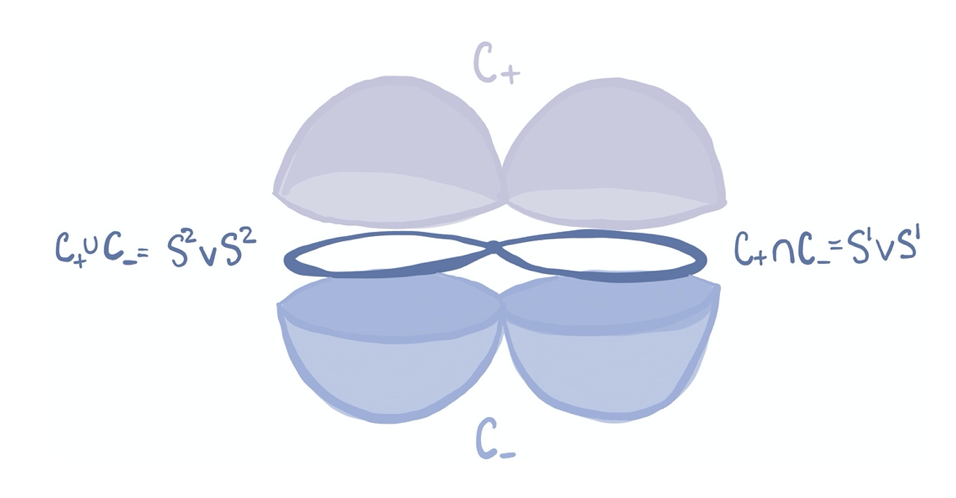
\includegraphics[scale = 0.5]{fst}\caption[][30pt]{The decomposition of $X = S^2 \vee S^2$ into the upper/lower hemispheres $C_{\pm}$, which intersect along the equator $S^1 \vee S^1$.}\label{fig:fst}\end{figure}


	 Then $C_+ \cap C_{-} \simeq S^1 \vee S^1$ and $C_+ \cup C_{-} = S^2 \vee S^2$. Note that both $C_+$ and $C_{-}$ are contractible (they have the homotopy type of a wedge of two discs). By the long exact sequence in homotopy we have 
	\[
\pi_i(S^2 \vee S^2,C_{-}) \cong \pi_i(S^2 \vee S^2) \quad \text{ and } \quad \pi_i(C_+,S^1 \vee S^2) \cong \pi_{i-1}(S^1 \vee S^2). 
	\]
	In particular, when $i = 2$ we have $\pi_2(S^2\vee S^2,C_{-}) \cong \pi_2(S^2 \vee S^2)$ is the free abelian group on two generators while $\pi_2(C_+,S^1 \vee S^1) \cong \pi_1(S^1 \vee S^1)$ is the free group on two generators. Therefore $(C_+,S^1 \vee S^1) \to (S^2 \vee S^2,C_{-})$ does not induce an isomorphism on homotopy. 
\end{Exa}
\begin{Rem}
The following is the homotopy theoretic version of excision. We will not give a full proof as it is quite involved. The full details can be found in May's book, for example. 
\end{Rem}
\begin{Thm}[Homotopy excision/Blakers--Massey theorem]\label{thm:excision}
	Let $(X;A,B)$ be an excisive triad such that $C = A \cap B$ is non-empty and $(A,C)$ and $(B,C)$ are relative CW-complexes. Suppose $(A,C,\ast)$ is $n$-connected and $(B,C,\ast)$ is $m$-connected for every choice of base-point $\ast \in C$. Then the map 
	\[
\pi_i(A,C) \to \pi_i(X,B)
	\]
	induced by the inclusion is an isomorphism for $i < n+m$ and a surjection for $i = n+m$, i.e., it is an $(n+m)$-equivalence. 
\end{Thm}
\begin{proof}[Sketch of proof]
	The proof proceeds by a number of reductions. 

	\textbf{Reduction 1: } It suffices to prove this when $A$ is built from $C$ by attaching cells of dimension greater than $n$ and $B$ is built by attaching cells of dimension greater than $m$. Indeed, we claim we can replace the pair $(A,C)$ with an $n$-connected pair $(A',C)$ such that the following diagram commutes: 
	% https://q.uiver.app/?q=WzAsMyxbMCwwLCJDIl0sWzEsMCwiQSciXSxbMCwxLCJBIl0sWzAsMSwiIiwwLHsic3R5bGUiOnsidGFpbCI6eyJuYW1lIjoiaG9vayIsInNpZGUiOiJ0b3AifX19XSxbMCwyLCIiLDIseyJzdHlsZSI6eyJ0YWlsIjp7Im5hbWUiOiJob29rIiwic2lkZSI6ImJvdHRvbSJ9fX1dLFsxLDIsIlxcc2ltIl1d
\[\begin{tikzcd}
	C & {A'} \\
	A
	\arrow[hook, from=1-1, to=1-2]
	\arrow[hook', from=1-1, to=2-1]
	\arrow["\sim", from=1-2, to=2-1]
\end{tikzcd}\]
and $A'$ is built from $C$ by attaching cells of dimension greater than $n$ only. To show this, we
build up a CW complex from $C$ by adding cells which represent elements of $\pi_i(A)$
or gets rid of elements which should not be there.\sidenote{For example, the first step is to kill the kernel of the surjection $\pi_n(C) \to \pi_n(A)$ by attaching cells to $A$. We will discuss this procedure in more detail when we discuss Eilenberg--Maclane spaces.} Since $\pi_i(C) \cong \pi_i(A)$ for all $i < n$, we only need to add cells of dimension greater than $n$ to make this work. This procedure can be carried out for $(B,C)$ as well.

\textbf{Reduction 2: } It suffices to prove excision when each of $A$ and $B$ is built from $C$ by attaching one cell apiece. To see this, let us say that a pair of extensions $C \to A$ and $C \to B$ is of size $(p,q)$ if $A$ is obtained by attaching $p$-cells (of dimension greater than $n$) and $B$ is obtained by attaching $q$-cells (of dimension greater than $m$). The claim is that excision holds for size $(1,1)$ if it holds for size $(p,q)$. The proof is inductive, via a long each sequence of `triad homotopy groups' and the 5-lemma.

The following lemma, whose proof is omitted, then completes the proof of homotopy excision. \end{proof}
\begin{Lem}Suppose that $X = A \cup_C B$ where $A = C \cup e$ and $B = C \cup e'$ are built from $C$ by attaching cells of dimension $>n$ and $>m$, respectively. Then, $\pi_i(A,C) \to \pi_i(X,B)$ is an isomorphism for $i < n+m$ and a surjection for $i = n+m$. 
\end{Lem}
Our main application will be the Freudenthal suspension theorem. We first make a definition. 
\begin{Def}
	Let $(X,x_0)$ be a based space. The suspension homomorphism is the map $\Sigma_* \colon \pi_i(X) \to \pi_{i+1}(\Sigma X)$ which sends $[f]$ to $[\Sigma f]$, where $\Sigma f \colon S^{i+1} \to \Sigma X$ sends $[s,t]$ to $[f(s),t]$. 
\end{Def}
\begin{Thm}
	Let $X$ be an $(n-1)$-connected CW-complex, then the suspension homomorphism
	\[
\Sigma_* \colon \pi_i(X) \to \pi_{i+1}(\Sigma X)
	\]
	is an isomorphism for $i < 2n-1$ and a surjection for $i = 2n-1$. 
\end{Thm}
\begin{proof}
	Write $\Sigma X = C_+X \cup C_{-}X$ for the decomposition of $\Sigma X$ into its upper and lower cone. Now consider the diagram
	% https://q.uiver.app/?q=WzAsNCxbMCwwLCJcXHBpX3tpKzF9KENfK1gsWCkiXSxbMSwwLCJcXHBpX3tpKzF9KFxcU2lnbWEgWCwgQ197LX1YKSJdLFswLDEsIlxccGlfaShYKSJdLFsxLDEsIlxccGlfe2krMX0oXFxTaWdtYSBYKSJdLFswLDFdLFswLDIsIlxcY29uZyIsMl0sWzIsMywiXFxTaWdtYV8qIiwyXSxbMSwzLCJcXGNvbmciXV0=
\[\begin{tikzcd}
	{\pi_{i+1}(C_+X,X)} & {\pi_{i+1}(\Sigma X, C_{-}X)} \\
	{\pi_i(X)} & {\pi_{i+1}(\Sigma X)}
	\arrow[from=1-1, to=1-2]
	\arrow["\cong"', "\partial", from=1-1, to=2-1]
	\arrow["{\Sigma_*}"', from=2-1, to=2-2]
	\arrow["\cong", "\partial"', from=1-2, to=2-2]
\end{tikzcd}\]
which can be shown to commute. Then it suffices to show that the upper diagram is an isomorphism/surjection in the appropriate range. To see this, note that if $X$ is $(n-1)$-connected, then $(C_{\pm}X,X)$ are $n$-connected (use the long exact sequence and contractibility of $C_{\pm}X$). By excision, 
\[
\pi_{i+1}(C_+,X) \to \pi_{i+1}(\Sigma X,C_{-}X)
\]
is an isomorphism for $ i + 1 < 2n$ and a surjection for $i+1 = 2n$, and the result follows.  
\end{proof}
\begin{Exa}
	The $n$-sphere has $\pi_i(S^n) = 0$ for $i < n$ (\Cref{exa:cellular_sphere}). So by the Freudenthal suspension theorem
	\[
\Sigma_* \colon \pi_i(S^n) \to \pi_{i+1}(S^{n+1})
	\]
	is an isomorphism for $i < 2n-1$. In particular, $\pi_n(S^n) \to \pi_{n+1}(S^{n+1})$ is an isomorphism for $n < 2n-1$, i.e., for $n \ge 2$. In particular, there is a surjection $\mathbb{Z} \cong \pi_1(S^1) \to \pi_2(S^2)$ and isomorphisms $\pi_2(S^2) \cong \pi_3(S^3) \cong \cdots \pi_n(S^n) $. In fact, the Hopf fibration $S^1 \to S^2 \to S^3$ shows that $\pi_2(S^2) \cong \mathbb{Z}$, and so we have $\pi_n(S^n) \cong \mathbb{Z}$ for all $n \ge 1$.  
\end{Exa}
\begin{Rem}
	Let $X$ be a CW-complex. By the suspension theorem $\Sigma^nX$ is always $(n+1)$-connected. Thus, 
	\[
\Sigma_* \colon \pi_i(\Sigma nX) \to \pi_{i+1}(\Sigma^{n+1}X)
	\]
	is an isomorphism for $i < 2n-1$. This means that for a fixed value of $k$, the maps in the sequence
	\[
\pi_k(X) \to \pi_{k+1}(\Sigma X) \to \pi_{k+2}(\Sigma^2X) \to \cdots \Sigma_{k+i}(\Sigma^iX)
	\]
	eventually become isomorphisms. This is known as the $k$-th stable homotopy group of $X$. 
\end{Rem}
\begin{Rem}
	There is an equivalent way to state homotopy excision. Suppose $f \colon A \to X$ is an $m$-equivalence and $g \colon A \to Y$ is an $n$-equivalence. We can form the following diagram
	% https://q.uiver.app/?q=WzAsNixbMSwwLCJBIl0sWzIsMCwiWCJdLFsxLDEsIlkiXSxbMiwxLCJaIl0sWzAsMCwiRl9mIl0sWzAsMSwiRl96Il0sWzAsMSwiZiJdLFswLDIsImciLDJdLFsyLDMsInoiLDJdLFsxLDNdLFszLDAsIiIsMSx7InN0eWxlIjp7Im5hbWUiOiJjb3JuZXItaW52ZXJzZSJ9fV0sWzQsMF0sWzUsMl0sWzQsNSwiXFx0aWxkZSBnIiwyLHsic3R5bGUiOnsiYm9keSI6eyJuYW1lIjoiZGFzaGVkIn19fV1d
\[\begin{tikzcd}
	{F_f} & A & X \\
	{F_z} & Y & Z
	\arrow["f", from=1-2, to=1-3]
	\arrow["g"', from=1-2, to=2-2]
	\arrow["z"', from=2-2, to=2-3]
	\arrow[from=1-3, to=2-3]
	\arrow["\ulcorner"{anchor=center, pos=0.125, rotate=180}, draw=none, from=2-3, to=1-2]
	\arrow[from=1-1, to=1-2]
	\arrow[from=2-1, to=2-2]
	\arrow["{\tilde g}"', dashed, from=1-1, to=2-1]
\end{tikzcd}\]
Then $\tilde f \colon F_f \to F_z$ is an $(n+m-1)$-equivalence. This follows because $\pi_n(X,A) \cong \pi_{n-1}F_f$ (use \Cref{thm:les_fibration} and the 5-lemma, for example). 
\end{Rem}
\begin{exercise}{}{}
Show that if $f \colon X \to Y$ is an $n$-connected map between spaces with $X$ an $(m-1)$-connected CW-complex, then the comparison map $F(f) \to \Omega C(f)$ is $(m+n-1)$-connected. 
\end{exercise}
\section{The CW-approximation theorem}
In this next section we show that, up to weak homotopy equivalence, every space is a CW-complex. We begin with the following. 
\begin{Lem}\label{lem:killing_cells}
Let $X$ be any space. Then there exists a space $Y$ and a map $i \colon X \to Y$ such that $i$ induces isomorphisms $\pi_q \colon \pi_qX \xrightarrow{\simeq} \pi_qY$ for $0 \le q \le n$ and $\pi_{n+1}Y = 0$.
\end{Lem}
\begin{proof}
The idea of the proof is to attach cells to $X$ to kill the classes we don't want to exist. To that end, let $J$ be a set of representatives for each $[j] \in \pi_{n+1}X$. Form the pushout diagram
% https://q.uiver.app/?q=WzAsNCxbMCwwLCJcXGNvcHJvZF97aiBcXGluIEp9U157bisxfSJdLFsxLDAsIlgiXSxbMCwxLCJcXGNvcHJvZF97aiBcXGluIEp9RF57bisyfSJdLFsxLDEsIlkiXSxbMCwxXSxbMCwyXSxbMiwzXSxbMSwzXSxbMywwLCIiLDEseyJzdHlsZSI6eyJuYW1lIjoiY29ybmVyLWludmVyc2UifX1dXQ==
\[\begin{tikzcd}[ampersand replacement=\&]
	{\coprod_{j \in J}S^{n+1}} \& X \\
	{\coprod_{j \in J}D^{n+2}} \& Y
	\arrow[from=1-1, to=1-2]
	\arrow[from=1-1, to=2-1]
	\arrow[from=2-1, to=2-2]
	\arrow[from=1-2, to=2-2]
	\arrow["\ulcorner"{anchor=center, pos=0.125, rotate=180}, draw=none, from=2-2, to=1-1]
\end{tikzcd}\]
Note that $(Y,X)$ is a relative CW-complex with  $Y^{n+1} = X$ so $X \to Y$ is an $(n+1)$-equivalence. We claim that $\pi_{n+1}Y = 0$. Indeed, let $f \colon (S^{n+1},\ast) \to (Y,\ast)$ be a representative of $\pi_{n+1}(Y)$. By cellular approximation we can assume that $f$ factors through the $(n+1)$-skeleton of $Y$, which is just $X$. In other words, $f \simeq j$ for some $j \in J$. But $j \colon S^{n+1} \to X \to Y$ is null-homotopic by assumption, and so $\pi_{n+1}Y = 0$.  
\end{proof}
\begin{Prop}[CW-approximation]
Given any topological space $X$ there exists a CW complex $\Gamma X$ and a weak equivalence $\Gamma X \xrightarrow{\gamma} X$.\footnote{In slightly fancy language, this is cofibrant replacement in a certain model structure on the category of topological spaces. }
\end{Prop}
\begin{proof}
We can assume that $X$ is path-connected, or we can work one path component at a time. Choose a set of representatives $J = \{ j_q \mid [j] \in \pi_qX, q \ge 1 \}$. Let $X_1 = \bigvee_{j_q \in J} S^q$ (with its standard CW structure) and $\gamma_1 \coloneqq \vee j_q \colon X_1 \to X$. By construction, $\gamma_1$ is a 1-equivalence. Suppose by induction that we have constructed a CW complex $X_n$ and an $n$-equivalence $X_n \to X$. Once again, let $J = \{ j \mid [j] \in \pi_nX_n, [\gamma_n \circ j] = 0 \in \pi_nX \}$. By construction, for each $j \in J$ there exists an extension $h_j$ of $S^n \xrightarrow{\gamma_n \circ j} X$ to $D^{n+1}$. We then construct $X_{n+1}$ by the pushout 	
% https://q.uiver.app/?q=WzAsNSxbMCwwLCJcXGNvcHJvZF97aiBcXGluIEp9U157bn0iXSxbMSwwLCJYIl0sWzAsMSwiXFxjb3Byb2Rfe2ogXFxpbiBKfURee24rMX0iXSxbMSwxLCJZIl0sWzIsMiwiWCJdLFswLDEsIlxcY29wcm9kIGoiXSxbMCwyXSxbMiwzXSxbMSwzXSxbMywwLCIiLDEseyJzdHlsZSI6eyJuYW1lIjoiY29ybmVyLWludmVyc2UifX1dLFsyLDQsIlxcY29wcm9kIGhfaiIsMix7ImN1cnZlIjoxfV0sWzEsNCwiXFxnYW1tYV9uIiwwLHsiY3VydmUiOi0xfV0sWzMsNCwiIiwyLHsic3R5bGUiOnsiYm9keSI6eyJuYW1lIjoiZGFzaGVkIn19fV1d
\[\begin{tikzcd}[ampersand replacement=\&]
	{\coprod_{j \in J}S^{n}} \& X_n \\
	{\coprod_{j \in J}D^{n+1}} \& X_{n+1} \\
	\&\& X
	\arrow["{\coprod j}", from=1-1, to=1-2]
	\arrow[from=1-1, to=2-1]
	\arrow[from=2-1, to=2-2]
	\arrow[from=1-2, to=2-2]
	\arrow["\ulcorner"{anchor=center, pos=0.125, rotate=180}, draw=none, from=2-2, to=1-1]
	\arrow["{\coprod h_j}"', curve={height=6pt}, from=2-1, to=3-3]
	\arrow["{\gamma_n}", curve={height=-6pt}, from=1-2, to=3-3]
	\arrow["{\gamma_{n+1}}", dashed, from=2-2, to=3-3]
\end{tikzcd}\]
Any map $S^q \to X_{n+1}$ for $q \le n$ factors through $X_n$, so $\pi_q\gamma_{n+1}$ factors through $\pi_q\gamma_n$ for $q \le n$. Since $X^n \to X^{n+1}$ is an $n$-equivalence, we have $\pi_q\gamma_{n+1} = \pi_q\gamma_n$ is an isomorphism for $0 \le q < n$. For $q = n$ we have a commutative diagram
% https://q.uiver.app/?q=WzAsMyxbMCwwLCJcXHBpX25YXm4iXSxbMSwwLCJcXHBpX3tufVhee24rMX0iXSxbMSwxLCJcXHBpX25YIl0sWzAsMSwiIiwwLHsic3R5bGUiOnsiaGVhZCI6eyJuYW1lIjoiZXBpIn19fV0sWzAsMiwiXFxwaV9uXFxnYW1tYV9uIiwyLHsic3R5bGUiOnsiaGVhZCI6eyJuYW1lIjoiZXBpIn19fV0sWzEsMiwiXFxwaV9uXFxnYW1tYV97bisxfSJdXQ==
\[\begin{tikzcd}[ampersand replacement=\&]
	{\pi_nX^n} \& {\pi_{n}X^{n+1}} \\
	\& {\pi_nX}
	\arrow[two heads, from=1-1, to=1-2]
	\arrow["{\pi_n\gamma_n}"', two heads, from=1-1, to=2-2]
	\arrow["{\pi_n\gamma_{n+1}}", from=1-2, to=2-2]
\end{tikzcd}\]
so that $\pi_n\gamma_{n+1}$ is a surjection. Moreover, any map $j \in \pi_nX^n$ such that $[\gamma_n \circ j] =0 \in \pi_{n+1}$ extends to $D^{n+1}$ in $X_{n+1}$, hence maps to zero in $\pi_{n+1}X_{n_1}$. Therefore, $\pi_n\gamma_{n+1}$ is also injective, and thus an isomorphism. 

Finally, setting $\Gamma X = \colim_n X_n$ and $\gamma= \colim_n \gamma_n$ gives the required CW-approximation.  
\end{proof}
\begin{Rem}
There is also a version of CW-approximation for pairs. Namely, if $(X,A)$ is pair then one can product a CW-pair $(\Gamma X,\Gamma A)$ weakly-homotopic to $(X,A)$ such that $\Gamma A$ is a sub-complex of $\Gamma X$. 
\end{Rem}
\begin{exercise}{}{}
Let $f \colon X \to Y$ be a map of topological spaces. Show that there is an induced map, $\Gamma f \colon \Gamma X \to \Gamma Y$, unique up to homotopy, between the CW-approximations to $X$ and $Y$, such that the following diagram commutes:
\[
% https://tikzcd.yichuanshen.de/#N4Igdg9gJgpgziAXAbVABwnAlgFyxMJZABgBpiBdUkANwEMAbAVxiRAB12BxOgW17oACABogAvqXSZc+QigCM5KrUYs2nHvyEBNcZJAZseAkTLzl9Zq0QhREqUdlFF56pbU3dY5TCgBzeCJQADMAJwheJDIQHAgkRRUrdW4+AUFgvRDwyMRo2KQAJjdVaw52P1S6EGoGOgAjGAYABWljORBQrD8ACxxMkDCI+Op8xABmYqSbTgqtfsGcopi48Zr6xpbHExtOnr7JjwHxCjEgA
\begin{tikzcd}
\Gamma X \arrow[r, "\Gamma f"] \arrow[d, "\gamma' "'] & \Gamma Y \arrow[d, "\gamma"] \\
X \arrow[r, "f"']                                   & Y                           
\end{tikzcd}.
\]
Deduce that CW-approximations are unique up to homotopy. 
\end{exercise}
\begin{exercise}{}{}
 Assume given maps $f \colon X \to Y$ and $g \colon Y \to X$ such that $g \circ f$ is
homotopic to the identity. (We say that $Y$ “dominates” $X$.) Suppose
that $Y$ is a CW complex. Prove that $X$ has the homotopy type of a CW
complex.
\end{exercise}
\section{Eilenberg--Maclane spaces}
\begin{Def}
A space $X$ having just one non-trivial homotopy group $\pi_n(X) = G$ is called an Eilenberg--MacLane space $K(G,n)$. 
\end{Def}
\begin{Exa}
We have seen that $S^1$ is a $K(\mathbb{Z},1)$ (\Cref{ex:s1}). We will see later that $\mathbb{C}P^{\infty}$ is a $K(\mathbb{Z},2)$. 
\end{Exa}
\begin{Rem}
We have not yet shown that Eilenberg--MacLane spaces exist in any generality. In fact, since $\pi_n$ is abelian for $n \ge 2$ we see that for $n \ge 2$ Eilenberg--Maclane spaces can only exist for $G$ abelian. The goal of this section is to show that this is the only obstruction: for any group $G$, abelian if $n \ge 2$, the Eilenberg--MacLane space $K(G,n)$ exists. We begin with a lemma. 
\end{Rem}
\begin{Lem}\label{lem:homotopy_wedge_spheres}
For $n \ge 2$ we have $\pi_n(\bigvee_{\alpha} S_{\alpha}^n)$ is free abelian, generated by the inclusion of the factors. 
\end{Lem}
\begin{proof}
Suppose first that we have only finitely many factors. Then we can regard $\bigvee_{\alpha} S_{\alpha}^n$ as the $n$-skeleton of $\prod_{\alpha} S_{\alpha}^n$. Taking the usual cell structure on $S^n$ we see that $\prod_{\alpha} S_{\alpha}^n$ has a cell structure with one zero cell and the $n$-cells 
\[
\bigcup_{\alpha}(\prod_{\beta \ne \alpha} D^0_{\beta}) \times D_{\alpha}^n
\]
and together these form the $n$-skeleton of  $\prod_{\alpha} S_{\alpha}^n$. Hence $\prod_{\alpha} S_{\alpha}^n \setminus \bigvee_{\alpha} S_{\alpha}^n$ has only cells of dimension at least $2n$, so that the pair $(\prod_{\alpha} S_{\alpha}^n,\bigvee_{\alpha} S_{\alpha}^n)$ is $(2n-1)$-connected by \Cref{cor:connectivity_cw_complex}. Therefore, we have (recall we fix $n \ge 2$)
\[
\pi_n(\bigvee_{\alpha} S_{\alpha}^n) \cong \pi_n(\prod_{\alpha} S_{\alpha}^n) \cong \prod_{\alpha} \pi_n(S_{\alpha}^n) \cong \bigoplus_{\alpha} \mathbb{Z}.
\]
This handles the case of finitely many summands. The infinite case can be reduced to this case in the following way: Let $\Phi \colon \bigoplus_{\alpha}\pi_n(S_{\alpha}^n) \to \pi_n(\bigvee_{\alpha} S_{\alpha}^n)$ be induced by the inclusions. Then, any map $f \colon S^n \to \bigvee_{\alpha} S_{\alpha}^n$ has compact image contained in the wedge of finitely many summands, so such that $[f]$ is in the image of $\Phi$ by the finite case, and $\Phi$ is surjective. Similarly, a null-homotopy of $f$ has compact image and again by the finite case $\Phi$ must be injective. 
\end{proof}
\begin{Rem}
If $n = 1$ then the Seifert--Van Kampen theorem shows that $\pi_1(\bigvee_{\alpha} S_{\alpha}^1)$ is the free group on the components; as soon as we have more than one sphere, this group is not abelian. 
\end{Rem}
\begin{Lem}\label{lem:technical_lemma}
	If a CW-pair $(X,A)$ is $r$-connected $(r \ge 1)$ and $A$ is $s$-connected $(s \ge 0)$, then the map $\pi_i(X,A) \to \pi_i(X/A)$ induced by the quotient map $X \to X/A$ is an isomorphism if $i \le r+s$ and onto if $i = r+s-1$. 
\end{Lem}
\begin{proof}
Let $i \colon A \to X$ be the inclusion and $C(i)$ the mapping cone, $C(i) = X \cup_A CA$. Since $CA$ is contractible and $(CA,C(i))$ is a cofibration the quotient map 
\[
q \colon C(i) \to C(i)/CA \simeq X/A
\]
is a homotopy equivalence (\Cref{thm:quotient_cofibration}). So we have a sequence of homomorphisms
\[
\pi_i(X,A) \to \pi_i(C(i),CA) \xleftarrow{\cong} \pi_i(C(i)) \xrightarrow{\cong} \pi_i(X/A),
\]
where the first and second maps are induced by the inclusion of pairs and the third map is the isomorphism $q_*$. The second map is an isomorphism by the long exact sequence of the pair $(C(i),CA)$. 

Now we know that $(X,A)$ is $r$-connected and $CA,A)$ is $(s+1)$-connected which follows from the assumption on $A$ on the long exact sequence in homotopy. The result now follows from excision, \Cref{thm:excision}. 
\end{proof}
\begin{Rem}
Suppose $n \ge 2$, and we are given maps $\phi_{\beta} \colon S_{\beta}^n \to \bigvee_{\alpha} S_{\alpha}^n$. Then we construct a space $X$ as the pushout 
% https://q.uiver.app/?q=WzAsNCxbMCwwLCJcXGJpZ3ZlZV97XFxiZXRhfSBTX3tcXGJldGF9Xm4iXSxbMSwwLCJcXGJpZ3ZlZV97XFxhbHBoYX0gU197XFxhbHBoYX1ebiJdLFswLDEsIlxcYmlndmVlX3tcXGJldGF9IERfe1xcYmV0YX1ee24rMX0iXSxbMSwxLCJYIl0sWzAsMSwiKFxccGhpX1xcYmV0YSkiXSxbMCwyLCIiLDIseyJzdHlsZSI6eyJ0YWlsIjp7Im5hbWUiOiJob29rIiwic2lkZSI6InRvcCJ9fX1dLFsyLDNdLFsxLDNdLFszLDAsIiIsMSx7InN0eWxlIjp7Im5hbWUiOiJjb3JuZXItaW52ZXJzZSJ9fV1d
\[\begin{tikzcd}[ampersand replacement=\&]
	{\bigvee_{\beta} S_{\beta}^n} \& {\bigvee_{\alpha} S_{\alpha}^n} \\
	{\bigvee_{\beta} D_{\beta}^{n+1}} \& X
	\arrow["{(\phi_\beta)}", from=1-1, to=1-2]
	\arrow[hook, from=1-1, to=2-1]
	\arrow["(\Phi_{\beta})"', from=2-1, to=2-2]
	\arrow[from=1-2, to=2-2]
	\arrow["\ulcorner"{anchor=center, pos=0.125, rotate=180}, draw=none, from=2-2, to=1-1]
\end{tikzcd}\]
\end{Rem}
\begin{Lem}
We have 
\[
\pi_n(X) \cong \pi_n(\bigvee_{\alpha} S_{\alpha}^n)/\langle \phi_{\beta} \rangle \cong (\bigoplus_{\alpha}\mathbb{Z})/\langle \phi_{\beta} \rangle.
\]
\end{Lem}
\begin{proof}
The pair $(X,\bigvee_{\alpha} S_{\alpha}^n)$ is $n$-connected and fits in a long exact sequence
\[
\pi_{n+1}(X,\bigvee_{\alpha} S_{\alpha}^n) \xrightarrow{\partial} \pi_n(\bigvee_{\alpha}S_{\alpha}^n) \to \pi_n(X) \to \pi_n(X,\bigvee_{\alpha} S_{\alpha}^n) = 0,
\]
where the final equality follows as a consequence of cellular approximation, see \Cref{cor:connectivity_cw_complex}. It follows that $\pi_n(X) \cong \pi_n(\bigvee_{\alpha}S_{\alpha}^n)/\im(\partial)$. 

We have $X/\bigvee_{\alpha} S_{\alpha}^n\simeq \bigvee S_{\beta}^{n+1}$, and so by \Cref{lem:homotopy_wedge_spheres} and \Cref{lem:technical_lemma} we have $\pi_{n+1}(X,\bigvee_{\alpha}S_{\alpha}^n) \cong \pi_{n+1}(\bigvee_{\beta} S_{\beta}^{n+1})$ is free with a basis consisting of the (restriction of the) characteristic maps $\Phi_{\beta}$ of the attaching cells. Since $\partial([\Phi_{\beta}]) = [\phi_{\beta}]$, the claim follows. 
\end{proof}
\begin{Exa}\label{Exa:almost_em_space}
Using the previous results, any abelian group $G$ can be realized as $\pi_n(X)$ for $n \ge 2$ of some space $X$. Indeed, choosing a presentation $G = \langle g_{\alpha} \mid r_{\beta} \rangle$ we can take
\[
X = \left ( \bigvee_{\alpha} S_{\alpha}^n \right) \cup \bigcup_{\beta} D_{\beta}^{n+1},
\]
with the $S_{\alpha}^n$'s corresponding to the generators, and the discs are attached by maps $f \colon S_{\beta}^n \to \bigvee_{\alpha}S_{\alpha}^n$ satisfying $[f] = r_{\beta}$. Then, the previous lemma says that $\pi_n(X) \cong G$. In fact, $\pi_i(X) = 0$ for $i < n$ by cellular approximation, but we have no control over the higher homotopy groups. In order to construct Eilenberg--Maclane spaces, we have to kill higher homotopy groups. 
\end{Exa}
\begin{Thm}
For any $n \ge 1$ and any group $G$ (abelian if $n \ge 2$) there exists an Eilenberg--Maclane space $K(G,n)$. 
\end{Thm}
\begin{proof}
Let $X_{n+1} = \left ( \bigvee_{\alpha} S_{\alpha}^n \right) \cup \bigcup_{\beta} D_{\beta}^{n+1}$ be as in \Cref{Exa:almost_em_space}. We want to build a space $X_{n+2}$ which agrees with $X_{n+1}$ in homotopy up to $\pi_n$ but has $\pi_{n+1}X_{n+2} = 0$. We have seen exactly how to do this in \Cref{lem:killing_cells}. Repeating this procedure inductively and taking colimits, we product a space $X$ with the correct homotopy groups. 
\end{proof}
\begin{exercise}{}{}
Exhibit a fibration $F \to E \to B$ where, up to weak homotopy equivalence, $F$ is a $K(G, n-1)$, $B$ is a $K(G,n)$ and $E$ is contractible.
\end{exercise}
\begin{Rem}
Eilenberg--Maclane spaces represent cohomology in the following sense.\footnote{We will talk about representability more when we discuss Brown representability}
\end{Rem}
\begin{Thm}\label{thm:representability_em}
There are natural bijections $T \colon [X,K(G,n)] \xrightarrow{\simeq} H^n(X;G)$ for all CW-complexes and all $n > 0$ with $G$ any abelian group. Such a $T$ has the form $T([f]) = f^*(\alpha)$ for a distinguished class $\alpha \in H^n(K(G,n);G)$.  
\end{Thm}
\begin{proof}
Recall that if $h^*$ is an unreduced cohomology theory on the category of CW-pairs, and $h^n(\ast) = 0$ for $n \ne 0$, then there exists a natural isomorphism $h^n(X,A) \cong H^n(X,A;h^0(\ast))$ for all CW-pairs $(X,A)$ and all $n$.

Now define $h^n(X) = [X,K(G,n)]$. This defines a reduced cohomology theory and the coefficient groups $h^n(S^i) = \pi_i(K(G,n)$ are the same as $\tilde H^i(S^i;G)$. Therefore, the previous paragraph (translated into reduced cohomology) gives the representability result. It remains to be seen that $T$ has the claimed form. This is formal: let $\alpha = T(\text{id})$ for $\text{id} \colon K(G,n) \to K(G,n)$ the identity map. Then, 
\[
T([f]) = T(f^*(\text{id})) \cong f^*(T(\text{id})) = f^*(\alpha). \qedhere
\]
\end{proof}
We can use this to prove a uniqueness theorem for Eilenberg--MacLane spaces. We begin with a lemma.
\begin{Lem}
If $X$ is $(n-1)$-connected, then $H^n(X;H) \cong \Hom(H_n(X);G)$.
\end{Lem}
\begin{proof}
This follows from a form of the Universal Coefficient theorem: there is an exact sequence
\[
0 \to \Ext(H_{n-1}(X),G) \to H^n(X;G) \to \Hom(H_n(X),G) \to 0,
\]
but the first term is zero by assumption. 
\end{proof}
\begin{Rem}
Let $G = \pi_n(X)$, then for $(n-1)$-connected $X$ the lemma gives $H^n(X;\pi_n(X)) \cong \Hom(H_n(X),\pi_n(X))$. The fundamental class $\iota$ is the class in $H^n(X;\pi_n(X))$ which corresponds to the inverse of a certain isomorphism $h_n \colon \pi_n(X) \cong H_n(X)$ we will construct in \Cref{sec:hurewicz}. In particular, to $K(G,n)$ we can associate a fundamental class $\iota_n \in H^n(K(G,n);G)$.
\end{Rem}
The following is a consequence of the representability of cohomology (\Cref{thm:representability_em}).
\begin{Cor}
There is a bijection
\[
[K(G,n),K(G',n)] \xrightarrow{\simeq} \Hom(G,G'). 
\]
\end{Cor}
\begin{proof}
We have bijections
\[
\begin{split}
	[K(G,n),K(G',n)] & \cong H^n(K(G,n);G') \\
	& \cong \Hom(H_n(K(G,n)),G') \\
	& \cong \Hom(G,G'). 
\end{split}
\]
\end{proof}
\begin{Cor}
The homotopy type of a CW-complex $K(G,n)$ is uniquely determined by $G$ and $n$.
\end{Cor}
\begin{proof}
If $G \cong G'$ then this can be realized by a map $K(G,n) \to K(G',n)$ by the previous corollary, and since all other homotopy groups are trivial, it follows from Whitehead's theorem that this map is a homotopy equivalence. 
\end{proof}
\begin{Rem}[Moore spaces]
There is a homology version of an Eilenberg--MacLane space, known as a Moore space: there exists a space $M(G,n)$ for an abelian group $G$ such that 
\[
\widetilde H_k(M(G,n)) \cong \begin{cases}
G & k = n \\
0 & \text{else.}
\end{cases}
\]
These can in fact be used to construct Eilenberg--MacLane spaces:\footnote{This is the Dold–Thom theorem.} Let $\Sp^n(X) \coloneqq X^{\times n}/\Sigma_n$, and let the infinite symmetric product of a space $X$, denoted $\Sp^{\infty}(X)$, be the colimit of the $\Sp^n(X)$. Then, for any connected space $X$, we have $\widetilde H_n(X) \cong \pi_n(\Sp^{\infty}(X)$. In particular, $\Sp^{\infty}(M(G,n))$ is the Eilenberg--MacLane space $K(G,n)$. 
\end{Rem}
\section{The Hurewicz theorem}\label{sec:hurewicz}
Define a homomorphism $h \colon \pi_i(X) \to H_i(X)$ by choosing a generator $u$ of $H_i(S^i) \cong \mathbb{Z}$ and defining $h([f]) = f_*(u)$. This is the Hurewicz homomorphism, and extends the Hurewicz homomorphism studied previously for $\pi_1$. 
\begin{Thm}
If a space $X$ is $(n-1)$-connected and $n \ge 2$, then $\tilde H_i(X) = 0$ for $i < n$ and $\pi_n(X) \cong H_n(X)$. Moreover, if a pair $(X,A)$ is $(n-1)$-connected with $n \ge 2$ and $\pi_i(A) = 0$, then $H_i(X,A) = 0$ for all $i \le n$ and $\pi_n(X,A) \cong H_n(X,A)$. 
\end{Thm}
\begin{Rem}
The isomorphism in the theorem is induced by $h_n$, but we do not show this. 
\end{Rem}
\begin{proof}
For note that the statements only involve homology and homotopy groups, so it suffices to use a CW approximation for $X$, or for $(X,A)$.\sidenote{Note that a weak equivalence in homotopy also induces a weak equivalence in (co)homology.} Secondly, the relative case can be reduced to the absolute case: $(X,A)$ is $(n-1)$-connected and $A$ is 1-connected, so \Cref{lem:whitehead_lemma} applies to show that $\pi_i(X,A) \cong \pi_i(X/A)$ for $i \le n$, while $H_i(X,A) \cong \tilde H_i(X/A)$ always holds for CW-pairs. 

By a version of CW-approximation, we can assume $X$ has $(n-1)$-skeleton a point. 	In particular, $\tilde H_i(X) = 0$ for $i < n$. For showing $\pi_n(X) \cong H_n(X)$ we may ignore cells of dimension $> n+1$ since these do not change $\pi_n$ or $H_n$. So we can assume $X = (\bigvee_{\alpha} S_{\alpha}^n) \cup \bigcup_{\beta} D_{\beta}^{n+1}$. As we have seen, we then have $\pi_n(X) \cong \oplus_{\alpha} \mathbb{Z}/\langle \phi_{\beta} \rangle$, and the same is true for $H_n(X)$ by cellular homology. 
\end{proof}
\begin{Cor}[The homology Whitehead theorem]
If $X$ and $Y$ are simply connected and $f \colon X \to Y$ a map inducing an isomorphism on homology, then $f$ is a homotopy equivalence. 
\end{Cor}
\begin{proof}
By using the mapping cylinder $M_f$ we can assume $f$ is an inclusion. Then by the long exact sequence in homology we have $H_n(Y,X) = 0$ for all $n$. Since $X$ and $Y$ are simply-connected $\pi_1(Y,X) = 0$. So by the relative Hurewicz theorem, the first non-zero $\pi_n(Y,X)$ is equal to the first non-zero $H_n(YmX)$. Therefore, $\pi_n(Y,X) = 0$ for all $n$. Therefore, $f_* \colon \pi_n(X) \to \pi_n(Y)$ is an isomorphism for all $n$. By Whitehead's theorem, $f$ is a homotopy equivalence. 
\end{proof}
\begin{exercise}{}{}
Show that a map between simply-connected CW complexes is a homotopy equivalence if its mapping cone is contractible. 
\end{exercise}
\begin{exercise}{}{}
 Show that a simply-connected closed 3-manifold is homotopy
equivalent to $S^3$. (You may assume that every closed manifold is homotopy equivalent to a CW-complex.)
\end{exercise}
\begin{Rem} This exercise is a little bit tricky, but you should try and compute the homology groups of such a manifold, and then use the homology Whitehead theorem. You should begin by noting that simply-connected manifolds are orientable. 
\end{Rem}
\section{Brown representability}
In this section we explain Brown's representability theorem, which one can use to give an abstract proof of \Cref{thm:representability_em}.\footnote{There are no proofs given in this section.}
\begin{Def}
Let $F \colon \mathcal C \to \Set$ be a functor. Then $F$ is representable if it is naturally isomorphic to $\Hom_{\mathcal C}(A,-)$ for some $A \in \mathcal C$. 
\end{Def}
\begin{Rem}
If such an $A$ exists, then it is unique up to unique isomorphism. 
\end{Rem}
\begin{Exa}
\begin{itemize}
\item The forgetful functor $\Ab \to \Set$ is representable. Indeed, $\Hom_{\Ab}(\mathbb{Z},M) \to M$ sending $f$ to $f(1)$ is an isomorphism. 
\item The forgetful functor $\Ring \to \Set$ is represented by $\mathbb{Z}[x]$: the map $\Hom_{\Ring}(\mathbb{Z}[x],M) \to M$ sending $f$ to $f(x)$ is a bijection. 
\item The functor $\Top^{\op} \to \Set$ that sends a topological space $(X,\tau_X)$ to its topology (the family of open sets) is representable. Indeed, let $Y = \{0 ,1\}$ with topology $\{ \emptyset, \{ 1 \}, \{ 0,1 \} \}$. Then, consider $\Hom_{\Top}(X,Y) \to \tau_X$ sending $f$ to $f^{-1}(\{ 1 \})$. This map is a bijection: the inverse is given by sending an open set $U$ to the characteristic function $\mathbb{1}_U$, i.e., the functor $\mathbb{1}_U \colon X \to \{ 0, 1\}$ defined by
\[
\mathbb{1}_U(x) = \begin{cases}
1, &x \in U\\
0, &x \not \in U.
\end{cases}
\]
\end{itemize}
\end{Exa}
\begin{Rem}
Note that representable functors preserve limits, because $\Hom_{\cat C}(A,-)$ preserves limits. This, if we want a functor to be representable it should at least preserve limits. Brown's representability theorem gives sufficient additional conditions for a functor from CW-complexes to Sets to be representable. 
\end{Rem}
Let $CW$ denote the homotopy category of based connected CW complexes. 
\begin{Thm}
	Let $F \colon CW^{\op} \to \Set$ be a functor satisfying:
	\begin{enumerate}
		\item $F(\bigvee_{\alpha} X_{\alpha}) = \prod_{\alpha} F(X_{\alpha})$
		\item Let $X$ be an object of CW. Consider a cover $X = Y \cup Z$ by sub-complexes such that $Y,Z,Y \cap Z \in CW$. Then, for all $y \in F(Y)$ and $z \in F(Z)$ that restrict to the same elect of $F(Y \cap Z)$, there exists some $x \in F(x)$ that restricts to $z \in F(Z)$ and $y \in F(Y)$.
	\end{enumerate}
	Then $F$ is representable: there exists some $C \in CW$ and $c \in F(c)$ such that for all $X \in CW$, the map
	\[
[X,C] \to F(x), f \mapsto f^*(c)
	\]
	is a bijection. 
\end{Thm}
\begin{Exa}
	Consider the functor $\tilde H^n(-;G) \colon CW^{\op} \to \Ab \to \Set$. This satisfies the above conditions (the second condition is essentially Mayer--Vietoris), and so there exists some $C \in CW$ and $c \in \widetilde H^n(C;G)$ such that 
		\[
[X,C] \to \widetilde H^n(X;G), f \mapsto f^*(c).
	\]
		is a bijection. In particular, if we take $X = S^i$, then 
	\[[S^i,C] = \pi_i(C) \cong \widetilde H^n(S^i;G) \cong \begin{cases}
	G & i = n \\
	0 & \text{otherwise.}
	\end{cases}
	\]
In other words, $C$ is a $K(G,n)$, and we recover \Cref{thm:representability_em}. 
\end{Exa}
\begin{Exa}
Let $X$ be \emph{any} space, and consider the functor $F_X \colon CW^{\op} \to \Set$ given by $Z \mapsto [Z,X]$. This is representable, and so there exists $Y \in CW$ and a map $f \colon Y \to X$ such that $[Z,Y] \xrightarrow{\cong} [Z,X]$. Taking $Z$ to be the spheres, we see that $Y \to X$ is a CW-approximation. 
\end{Exa}
\end{document}
